\documentclass[
  aps,
  prd,
  twocolumn,
  amsmath,
  amssymb,
  nofootinbib,
  superscriptaddress,
  floatfix,
]{revtex4-2}

\usepackage{graphicx}
\usepackage{booktabs}
\usepackage{xcolor}
\usepackage{hyperref}
\hypersetup{colorlinks=true, linkcolor=blue, citecolor=blue, urlcolor=blue}

\graphicspath{{figures/}}

% --- editorial placeholder marker (remove before submission) ---
\newcommand{\todo}[1]{{\color{red}\textbf{[TODO: #1]}}}
\newcommand{\stub}[1]{{\color{gray}\textit{[#1]}}}

% --- convenient macros ---
\newcommand{\psiBL}{\psi_{\mathrm{BL}}}
\newcommand{\Ahat}{\hat{A}}
\newcommand{\dID}{\partial \mathrm{ID}/\partial\theta}
\newcommand{\Madm}{M_{\mathrm{ADM}}}

\begin{document}

% ===========================================================================
%  TITLE / AUTHOR BLOCK  --  USER-OWNED.  Do not auto-fill.
% ===========================================================================
\title{A Certified and Differentiable Parametric Solver \\ for Binary-Black-Hole Puncture Initial Data}

\author{Frederik De Ceuster}
\email{frederik.deceuster@kuleuven.be}
\affiliation{Institute for Theoretical Physics, KU Leuven, Celestijnenlaan 200D, 3001 Leuven, Belgium}
\affiliation{Leuven Gravity Institute, KU Leuven, Celestijnenlaan 200D, 3001 Leuven, Belgium}
\affiliation{STADIUS Center for Dynamical Systems, Signal Processing and Data Analytics, KU Leuven, Kasteelpark Arenberg 10, 3001 Leuven, Belgium}

\author{Tjonnie G.-F. Li}
\affiliation{Institute for Theoretical Physics, KU Leuven, Celestijnenlaan 200D, 3001 Leuven, Belgium}
\affiliation{Leuven Gravity Institute, KU Leuven, Celestijnenlaan 200D, 3001 Leuven, Belgium}
\affiliation{STADIUS Center for Dynamical Systems, Signal Processing and Data Analytics, KU Leuven, Kasteelpark Arenberg 10, 3001 Leuven, Belgium}

\date{\today}

\begin{abstract}
Constraint-satisfying initial data for binary black holes require the repeated solution of a nonlinear elliptic boundary-value problem throughout the physical parameter space.
We present a parametric initial-data solver that combines sparse-grid spectral interpolation with Newton refinement to construct certified, differentiable initial data over a chosen family of binary configurations.
Interpolation is used only to provide warm starts for the underlying elliptic solver, rather than to replace it.
A small number of Newton iterations refines each interpolated solution to a constraint residual $\|R\|_\infty\le10^{-10}$, independent of the interpolation error, thereby certifying every generated initial-data set.
A JAX implementation further provides derivatives of the certified initial data with respect to the physical parameters, enabling gradient-based parameter targeting, optimization, and sensitivity analysis.
We demonstrate the method for quasi-circular binary-black-hole puncture initial data by constructing four-dimensional aligned-spin and eight-dimensional general-spin models.
The resulting initial data are validated against TwoPunctures, and the method is applied to certified targeting of the physical ADM mass and angular momentum and to effective-potential eccentricity reduction using a dedicated $(b,P_t)$ model.
\end{abstract}

\maketitle

% ===========================================================================
\section{Introduction}
\label{sec:intro}
% ===========================================================================
Every numerical-relativity simulation of a binary black hole begins by solving the Einstein constraint equations on the initial time slice.
For conformally flat, maximally sliced puncture data, this reduces to a nonlinear elliptic boundary-value problem: the Lichnerowicz--York form of the Hamiltonian constraint for the conformal factor~\cite{York1979,BowenYork1980,BrandtBruegmann1997,Cook2000}.
This problem must be solved once for each physical configuration.


Modern applications, however, rarely require a single solution.
Parameter surveys, waveform catalogs, eccentricity reduction, and mass and spin targeting all require the same elliptic problem to be solved repeatedly across the physical parameter space of binary black holes.
The repeated solution of the constraint equations therefore becomes the dominant recurring computational cost~\cite{Mendes2025}.
The computational challenge is therefore not solving a single elliptic problem, but efficiently solving a family of closely related elliptic problems across the physical parameter space.


Reduced-order modeling is a mature response to exactly this kind of repeated computation.
In gravitational-wave physics, however, it has been developed almost exclusively for \emph{waveforms}: reduced-basis template banks and surrogate models reproduce waveforms across parameter space at a tiny fraction of the cost~\cite{FieldGalley2011,Field2014,Blackman2015,Varma2019}.
The elliptic initial-data solve that precedes every numerical-relativity evolution has largely remained outside this development.
Reduced-basis emulation does exist for the neutron-star sector, for example through Tolman--Oppenheimer--Volkoff emulators over equation-of-state parameters~\cite{Reed2024}, but no comparable parametric solver exists for binary-black-hole puncture initial data.


From the perspective of numerical analysis, this gap is somewhat surprising.
Parametric collocation, sparse interpolation, and reduced-basis methods for parameter-dependent elliptic partial differential equations are well-established~\cite{BabuskaNobileTempone2007,XiuHesthaven2005,NobileTemponeWebster2008,Haasdonk2017,HesthavenRozzaStamm2016}.
When the parameter-to-solution map is analytic, the interpolation error decays exponentially with the number of parameter samples at a rate determined by the nearest singularity in the complex parameter plane through the Bernstein-ellipse estimate~\cite{Trefethen2019}.
These results suggest that binary-black-hole puncture initial data should also admit efficient parametric representations over suitable regions of parameter space.


Several recent developments have addressed complementary aspects of this problem.
Mendes \emph{et al.}~\cite{Mendes2025} accelerate parameter targeting through a Broyden iteration that repeatedly re-solves the constraint equations.
Tommasini \emph{et al.}~\cite{Tommasini2026} use Gaussian-process regression trained on the SXS catalogue to predict low-eccentricity orbital parameters, reducing the number of trial evolutions required for eccentricity reduction.
Zhou \emph{et al.}~\cite{Zhou2026} introduce a physics-informed neural-network solver for the puncture Hamiltonian constraint on a single configuration and identify parameterized initial-data solvers as an important direction for future work.
Analytic perturbative constructions~\cite{Ogurol2025} and neural representations of spacetime metrics~\cite{Cranganore2025} provide additional complementary approaches.
None of these methods, however, simultaneously constructs a parametric solver, certifies the constraint satisfaction of every returned solution, and provides exact derivatives of the resulting initial data with respect to the physical parameters.


This paper addresses this gap by introducing a parametric solver for binary-black-hole puncture initial data with certified constraint satisfaction and exact differentiability with respect to the physical parameters.
Rather than replacing the elliptic solve with an approximation, the method constructs a sparse interpolant that provides a high-quality initial guess for the nonlinear solve, after which a small number of Newton iterations recover a fully converged solution satisfying the Einstein constraint equations.
We demonstrate the approach for both a four-dimensional aligned-spin model and an eight-dimensional general-spin quasi-circular model, and apply it to two representative tasks: targeting physical parameters and reducing orbital eccentricity.


The proposed solver combines three properties that, to our knowledge, have not previously been demonstrated together for binary-black-hole puncture initial data: it is parametric, provides certified constraint satisfaction, and is exactly differentiable with respect to the physical parameters.
First, it provides \emph{certified constraint satisfaction}. Every queried parameter is refined by Newton iterations until the constraint residual satisfies $\|R\|_\infty \le 10^{-10}$, ensuring that every returned initial datum satisfies the Einstein constraints to a prescribed tolerance.
The sparse interpolant therefore accelerates the computation but does not replace the underlying elliptic solver.
Second, it provides \emph{exact differentiability}.
The entire construction is implemented in JAX~\cite{Jax2018}, making the resulting parameter-to-solution map exactly differentiable with respect to the physical parameters.
These derivatives are obtained automatically through algorithmic differentiation without finite-difference approximations or adjoint implementations.


The remainder of this paper is organized as follows.
Section~\ref{sec:problem} reviews the puncture initial-data formulation and the resulting nonlinear elliptic constraint equation.
Section~\ref{sec:solve} describes the spectral elliptic solver that produces a single constraint-satisfying datum.
Section~\ref{sec:param} builds the parametric solver over it, combining sparse interpolation, Newton refinement that certifies every returned datum, and a differentiable JAX implementation.
Section~\ref{sec:model} constructs and characterizes the four-dimensional aligned-spin and eight-dimensional general-spin quasi-circular models, including their convergence and the analyticity limits of the parameter map.
Section~\ref{sec:applications} applies the method to certified parameter targeting and effective-potential eccentricity reduction.
Finally, Section~\ref{sec:conclusions} discusses the limitations, implications, and conclusions of this work.
Validation of the underlying initial data against TwoPunctures is collected in Appendix~\ref{sec:validation}.




% This paper closes that gap. We present a parametric and differentiable model for the
% binary-black-hole initial-data problem, i.e.\ a recipe that yields a differentiable, constraint-certified surrogate over any
% chosen family of binaries, and demonstrate it with a 4-dimensional (aligned-spin) and an 8-dimensional (general-spin) quasi-circular model.
% Moreover, we present two applications of the machinery: targeting physical parameters and reducing orbital eccentricity.
% To our knowledge, it is the first reduced-order, parametric treatment of BBH initial data; with two key features:
% \begin{enumerate}
% \item It is \emph{certified}. The interpolant supplies only an initial
%   guess after which a few Newton iterations of the genuine elliptic solver drive the
%   constraint residual to $\|R\|_\infty \le 10^{-10}$ at any queried parameter.
%   As a result, this surrogate cannot be silently wrong:
%   every datum it emits satisfies the constraints to a checked tolerance.
%   This makes it more than
%   ``TwoPunctures~\cite{AnsorgBruegmannTichy2004} plus interpolation''.
%   Our elliptic solver is a re-implementation of TwoPunctures,
%   but the key contribution is the parametric, differentiable, and
%   certified \emph{parameter map} built over it.

% \item It is \emph{differentiable}. Implemented in JAX~\cite{Jax2018}, it exposes
%   the gradient of the (interpolated, certified) initial data with
%   respect to the physical parameters, enabling gradient-based parameter
%   targeting and sensitivity analysis. This is the ingredient a black-box solver
%   cannot supply, and we show it changes the cost of real initial-data workflows:
%   hitting a physical target, or reducing orbital eccentricity, in a few certified
%   solves where a black box needs many.
% \end{enumerate}

% Furthermore, we make the limits of the method \emph{quantitative}.
% We measure the analyticity walls, i.e.\ the degradation of the convergence rate as the binary parameters approache merger
% and as the spins increase, and we match each to its theoretical (Bernstein-ellipse) prediction.


% Our headline models are \emph{quasi-circular} orbiting black-hole binaries.
% We fix the tangential and radial momenta by a post-Newtonian quasi-circularity
% condition, so that every point of
% the parameter space is a physical orbiting configuration rather than a free
% momentum knob. The physical parameters are then the mass ratio $q$, the coordinate
% separation $b$ (equivalently the orbital frequency), and the two spin vectors
% $\boldsymbol{S}_{A},\boldsymbol{S}_{B}$ (or their dimensionless counterparts $\boldsymbol{\chi}_{A},\boldsymbol{\chi}_{B}$), while the initial slice is assumed to be conformally flat and maximally sliced.

% The paper is organized as follows. Section~\ref{sec:problem} states the puncture
% initial-data problem, Section~\ref{sec:solve} describes the initial-data solver, and
% Section~\ref{sec:param} presents the methodology for building the parametric
% surrogate.
% Section~\ref{sec:model} then shows the quasi-circular model, including the analyticity results, which are validated in Appendix~\ref{sec:validation} against TwoPunctures.
% Section~\ref{sec:applications} sketches two applications: physical parameter targeting and eccentricity reduction, and Section~\ref{sec:conclusions} discusses limitations and outlook.

% ===========================================================================
\section{Puncture initial data}
\label{sec:problem}
% ===========================================================================
We briefly review the puncture formulation of binary-black-hole initial data used
throughout this work. We adopt conformally flat, maximally sliced initial data
within York's conformal transverse--traceless
decomposition~\cite{York1979,Cook2000}, rather than the conformal thin-sandwich
formulation~\cite{York1999}. Under these assumptions, the momentum constraint is
satisfied analytically, leaving a single nonlinear elliptic equation for the
conformal factor.

\subsection{Constraint and puncture decomposition}
\label{sec:problem:decomp}

In the conformal decomposition, the spatial metric and extrinsic curvature are
$\gamma_{ij} = \psi^4 f_{ij}$ and $K^{ij} = \psi^{-10}\Ahat^{ij}$, where
$f_{ij}$ is the flat conformal metric and $\Ahat^{ij}$ is the conformal
(Bowen--York) extrinsic curvature. We assume maximal slicing,
$K\equiv f_{ij}K^{ij}=0$. If $\Ahat^{ij}$ is transverse with respect to the flat
metric, $\partial_i\Ahat^{ij}=0$, the momentum constraint is satisfied
analytically (Sec.~\ref{sec:problem:source}), while the Hamiltonian constraint
reduces to the nonlinear Lichnerowicz--York equation
\begin{equation}
  \Delta \psi \ = \ -\tfrac{1}{8}\, \psi^{-7}\, \Ahat_{ij}\Ahat^{ij},
  \label{eq:lichnerowicz}
\end{equation}
where $\Delta$ is the flat Laplacian and indices are raised and lowered with
$f_{ij}$. This is the only equation that must be solved numerically.

Equation~\eqref{eq:lichnerowicz} is defined on an unbounded domain and is
singular at each puncture because $\Ahat^2$ diverges there. Following Brandt and
Br\"ugmann~\cite{BrandtBruegmann1997}, we decompose the conformal factor as
$\psi=\psiBL+u$, where the $N$-puncture Brill--Lindquist background is
\begin{equation}
  \psiBL \ = \ 1 + \sum_{X} \frac{m_X}{2 r_X},
  \label{eq:psiBL}
\end{equation}
where $r_X \equiv |\mathbf{x}-\mathbf{x}_X|$ is the coordinate distance to
puncture $X$. The Brill--Lindquist term contains all $1/r_X$ singularities and
is harmonic away from the punctures. The regular correction therefore satisfies
\begin{equation}
  \Delta u \ = \ -\tfrac{1}{8}\,(\psiBL + u)^{-7}\, \Ahat_{ij}\Ahat^{ij},
  \label{eq:u_eq}
\end{equation}
where, for the binary, we take $N=2$ punctures of bare masses $m_A$ and $m_B$
located at $z=\pm b$. Solving Eq.~\eqref{eq:u_eq} for $u$ determines the
complete initial data.


\subsection{Bowen--York source term}
\label{sec:problem:source}
The momentum constraint is satisfied analytically by the Bowen--York extrinsic
curvature~\cite{BowenYork1980},
\begin{align}
  \Ahat^{ij} \ &= \ \sum_{X\in\{A,B\}} \bigl(\Ahat^{ij}_{P,X} + \Ahat^{ij}_{S,X}\bigr),
\end{align}
where the momentum and spin contributions are
\begin{align}
  \Ahat^{ij}_{P,X} \ &\equiv \ \frac{3}{2 r_X^2}\Bigl[
  P_X^i n_X^j + P_X^j n_X^i \nonumber \\
  & \hspace{15mm} - \bigl(f^{ij} - n_X^i n_X^j\bigr)(\mathbf{P}_X\!\cdot\!\mathbf{n}_X)\Bigr],
  \label{eq:A_P}
  \\
  \Ahat^{ij}_{S,X} \ &\equiv \ \frac{3}{r_X^3}\bigl(v_X^i n_X^j + v_X^j n_X^i\bigr),
  \label{eq:A_S}
\end{align}
where $\mathbf{P}_X$ and $\mathbf{S}_X$ are the linear momentum and spin of
puncture $X$, respectively,
$\mathbf{v}_X \equiv \mathbf{S}_X\times\mathbf{n}_X$, and
$\mathbf{n}_X \equiv (\mathbf{x}-\mathbf{x}_X)/r_X$ is the unit
radial vector centered on puncture $X$. The tensor $f^{ij}$ in Eq.~\eqref{eq:A_P} is the inverse flat
conformal metric; in the Cartesian coordinates used to construct the tensor,
$f^{ij}=\delta^{ij}$. Each Bowen--York contribution is transverse and
trace-free with respect to $f_{ij}$. Their sum therefore satisfies the momentum
constraint analytically for arbitrary momenta, spins, and separations.

The Hamiltonian constraint depends only on the scalar contraction
$\Ahat_{ij}\Ahat^{ij}$. Defining
$\Ahat_X \equiv \Ahat_{P,X}+\Ahat_{S,X}$ as the total tensor associated with
puncture $X$, the contraction decomposes into two self-contractions and a cross
term,
\begin{equation}
  \Ahat_{ij}\Ahat^{ij} \ = \ \Ahat_A\!:\!\Ahat_A \;+\; 2\,\Ahat_A\!:\!\Ahat_B \; + \; \Ahat_B\!:\!\Ahat_B .
  \label{eq:A2_full}
\end{equation}
Each self-contraction is
\begin{equation}
\begin{aligned}
  \Ahat_X\!:\!\Ahat_X \ = \ &
  \frac{9}{2r_X^4}\bigl[P_X^2 \, + \, 2(\mathbf{P}_X\!\cdot\!\mathbf{n}_X)^2\bigr] \\
  &+ \frac{18}{r_X^6}\,|\mathbf{S}_X\!\times\!\mathbf{n}_X|^2
   + \frac{18}{r_X^5}\,(\mathbf{P}_X\!\times\!\mathbf{S}_X)\!\cdot\!\mathbf{n}_X ,
\end{aligned}
  \label{eq:A2_self}
\end{equation}
where the three terms are the momentum, spin, and momentum--spin contributions,
respectively. The cross term is
\begin{equation}
\begin{aligned}
  2\,\Ahat_A\!:\!\Ahat_B \ = \ &
  \frac{9}{2r_A^2 r_B^2}\,\Pi_{AB}
  \ + \ \frac{36}{r_A^3 r_B^3}\,\Sigma_{AB} \\
  &+ \ \frac{18}{r_A^2 r_B^3}\,\Xi_{AB}
  \ + \ \frac{18}{r_A^3 r_B^2}\,\Xi_{BA} ,
\end{aligned}
  \label{eq:A2_cross}
\end{equation}
where the momentum--momentum ($\Pi$), spin--spin ($\Sigma$), and
momentum--spin ($\Xi$) invariants are
\begin{align}
  \Pi_{AB} \ &\equiv \ 2(\mathbf{P}_A\!\cdot\!\mathbf{n}_B)(\mathbf{P}_B\!\cdot\!\mathbf{n}_A)
   - 3(\mathbf{P}_A\!\cdot\!\mathbf{n}_A)(\mathbf{P}_B\!\cdot\!\mathbf{n}_B) \nonumber\\
  &\hspace{5mm} + 2(\mathbf{n}_A\!\cdot\!\mathbf{n}_B)\bigl[ (\mathbf{P}_A\!\cdot\!\mathbf{P}_B) \nonumber \\
  &\hspace{25mm} + (\mathbf{P}_A\!\cdot\!\mathbf{n}_A)(\mathbf{P}_B\!\cdot\!\mathbf{n}_A) \nonumber\\
  &\hspace{25mm} + (\mathbf{P}_B\!\cdot\!\mathbf{n}_B)(\mathbf{P}_A\!\cdot\!\mathbf{n}_B)\bigr] \nonumber\\
  &\hspace{ 5mm} + (\mathbf{P}_A\!\cdot\!\mathbf{n}_A)(\mathbf{P}_B\!\cdot\!\mathbf{n}_B)(\mathbf{n}_A\!\cdot\!\mathbf{n}_B)^2 ,
  \label{eq:invPi}\\
  \Sigma_{AB} \ &\equiv \ (\mathbf{v}_A\!\cdot\!\mathbf{v}_B)(\mathbf{n}_A\!\cdot\!\mathbf{n}_B) + (\mathbf{v}_A\!\cdot\!\mathbf{n}_B)(\mathbf{v}_B\!\cdot\!\mathbf{n}_A) ,
  \label{eq:invSigma}\\
  \Xi_{AB} \ &\equiv \ (\mathbf{P}_A\!\cdot\!\mathbf{v}_B)(\mathbf{n}_A\!\cdot\!\mathbf{n}_B)
   + (\mathbf{P}_A\!\cdot\!\mathbf{n}_B)(\mathbf{n}_A\!\cdot\!\mathbf{v}_B) \nonumber\\
  & \hspace{5mm} + (\mathbf{P}_A\!\cdot\!\mathbf{n}_A)(\mathbf{n}_A\!\cdot\!\mathbf{n}_B)(\mathbf{n}_A\!\cdot\!\mathbf{v}_B) ,
  \label{eq:invXi}
\end{align}
where $\Xi_{BA}$ follows from exchanging $A$ and $B$.


\subsection{Regularity of the puncture formulation}
\label{sec:problem:regularity}
The puncture decomposition isolates the singular part of the conformal factor in the analytic Brill--Lindquist background $\psiBL$.
Near puncture $X$, $\psiBL^{-7}\sim r_X^7$, whereas the momentum and spin self-contractions scale as $\Ahat_{P,X}^2\sim r_X^{-4}$ and $\Ahat_{S,X}^2\sim r_X^{-6}$, respectively.
Hence, their contributions to the effective source in Eq.~\eqref{eq:u_eq} vanish at least linearly as $r_X\to0$.
The cross terms are likewise regular and vanish at the puncture.
Consequently, $u$ is smooth throughout the compactified computational domain, making it well suited to the spectral discretization introduced in Sec.~\ref{sec:solve}.



% ===========================================================================
\section{Constraint solver}
\label{sec:solve}
% ===========================================================================
We solve Eq.~\eqref{eq:u_eq} for the regular correction $u$ by spectral collocation on a single spectral patch.
We use the Ansorg--Br\"ugmann--Tichy (TwoPunctures) spectral method~\cite{AnsorgBruegmannTichy2004}, extended with a Fourier expansion in $\phi$ for non-axisymmetric configurations.
This solver provides the reference solution on which the parametric method of Sec.~\ref{sec:param} is built and against which it is validated.


\subsection{The prolate-spheroidal single patch}
\label{sec:solve:abt}

The Ansorg--Br\"ugmann--Tichy (ABT) coordinate system~\cite{AnsorgBruegmannTichy2004} maps the two-puncture domain onto a single compact spectral patch.
Starting from cylindrical coordinates $(\rho,z,\phi)$, it introduces prolate-spheroidal coordinates whose foci coincide with the punctures at $z=\pm b$, together with a compactified radial coordinate.
With $A\in[0,1]$ and $B\in[-1,1]$, the transformation to cylindrical coordinates is
\begin{equation}
  \frac{\rho}{b} = \frac{2A\sqrt{1-B^2}}{1-A^2}, \qquad
  \frac{z}{b}   = \frac{(1+A^2)\,B}{1-A^2}.
  \label{eq:abt_map}
\end{equation}
The coordinate edges have a
clean meaning: $A=1$ is spatial infinity, $A=0$ is the inner axis segment
$|z|\le b$, the edges $B=\pm1$ are the outer axis $|z|\ge b$, and the two corners
$(A=0,B=\pm1)$ are the punctures themselves.

Because the ABT coordinates are orthogonal, the flat-space Laplacian takes the separable form
\begin{equation}
\begin{aligned}
   \Delta u \ &= \ \frac{(1-A^2)^2}{b^2\,\mathcal{D}} \bigg[
    \frac{(1-A^2)^2}{4A}\,\partial_A\!\big(A\,\partial_A u\big) \\
    &\hspace{23mm} \, + \, \partial_B\!\big[(1-B^2)\,\partial_B u\big]\bigg]
     + \frac{\partial_{\phi}^2 u}{\rho^{2}},
\end{aligned}
  \label{eq:abt_laplacian}
\end{equation}
with $\mathcal{D} \equiv (1+A^2)^2 - B^2(1-A^2)^2$ and $\rho$ from
Eq.~\eqref{eq:abt_map}.


In a Fourier basis in $\phi$, the azimuthal derivative diagonalizes, $\partial_\phi^2\!\rightarrow\!-m^2$, so each Fourier mode can be treated independently.
The linear Lichnerowicz operator therefore decomposes into independent two-dimensional blocks, eliminating the need to assemble the full three-dimensional dense matrix.


The regular correction is represented nodally: the unknown is the tensor of collocation values $U_{ijk}\equiv u(A_i,B_j,\phi_k)$, rather than the modal coefficients ($c^{m}_{nl}$ below).
This representation is equivalent to the truncated spectral expansion
\begin{equation}
  u(A,B,\phi) = \!\!\sum_{|m|\le N_\phi/2} \ \sum_{n=0}^{N_A}\sum_{l=0}^{N_B-1} c^{m}_{nl} \ \phi_{nl}^{m}(A,B,\phi) \label{eq:expansion}
\end{equation}
with basis functions,
\begin{equation}
  \phi_{nl}^{m}(A,B,\phi) \equiv T_n(2A-1)\,P_l(B) \, e^{im\phi}\,(1-B^2)^{|m|/2} .
  \label{eq:basis}
\end{equation}
The basis consists of a Fourier expansion in the azimuthal angle $\phi$, (with $c^{-m}_{nl}=(c^{m}_{nl})^{*}$ since
$u$ is real), Chebyshev polynomials $T_n$ in the compactified radial coordinate
$A$, and Legendre polynomials $P_l$ in the angle $B$. The associated-Legendre
prefactor $(1-B^2)^{|m|/2}$ carries the exact behaviour of the regular $m$-mode at
the outer axis $B=\pm1$. For odd $m$ this yields a square-root branch point that a bare
polynomial can only resolve algebraically, so we solve for the smooth polynomial
factor and differentiate the prefactor analytically, restoring spectral
convergence for every mode. 
The coefficients $c_{nl}^m$ are not formed explicitly.
The azimuthal FFT maps the $N_\phi$ node values to the modes $m$, and within each meridian block the $A$- and $B$-derivatives act on the nodal values through the Chebyshev and Legendre differentiation matrices.

A solved field must also be evaluated \emph{off} the collocation grid at
arbitrary coordinates $(A,B,\phi)$. Although this could be done by forming the
coefficients $c^{m}_{nl}$ and evaluating the expansion in
Eq.~\eqref{eq:expansion}, we instead interpolate the nodal values directly. We
use the numerically stable barycentric-Lagrange
formula~\cite{Trefethen2019} in $A$ and $B$, applied to the smooth polynomial
factor with the analytic $(1-B^2)^{|m|/2}$ prefactor restored for each mode, and
equispaced trigonometric interpolation in $\phi$. This procedure is not an
approximation to the truncated spectral representation: the barycentric
interpolant is the unique polynomial of the retained degree passing through the
collocation values, while the trigonometric interpolant is the corresponding
unique band-limited periodic interpolant. Consequently, the interpolated field
is mathematically identical to the truncated expansion of
Eqs.~\eqref{eq:expansion} and~\eqref{eq:basis}, evaluated in a
coefficient-free form.

We place Chebyshev--Gauss--Lobatto nodes in $A$ ($N_A{+}1$ nodes, with
$A{=}1$ at spatial infinity and $A{=}0$ on the inner axis) and Gauss--Legendre
nodes in $B$ ($N_B$ interior nodes that avoid the polar edges $B=\pm1$ and, being a
full nodal grid, carry both $z$-parities). Boundary conditions are imposed by
row-replacement: Dirichlet $u=0$ at the $A=1$ (infinity) edge and Neumann
$\partial_A u = 0$ on the $A=0$ inner axis; on that inner axis only the $m=0$ mode
is regular, so we impose $u_m=0$ there for $m\neq0$, consistent with the $m=0$
Neumann row. The Laplacian's rows span a huge
dynamic range: the $(1-A^2)^4$ factor is tiny near infinity and the $1/A$ factor
large near the inner axis, giving a raw condition number $\sim10^{13}$--$10^{15}$.
Using row equilibration, i.e.\ scaling each row by $1/\max_j|M_{ij}|$, an exact
rescaling of the equations that leaves the solution unchanged, collapses the
condition number to $\sim10^4$ and takes the solve to machine precision.


\subsection{Newton iteration with an analytic Jacobian}
\label{sec:solve:newton}

We solve Eq.~\eqref{eq:u_eq} for the nodal field
$U_{ijk}=u(A_i,B_j,\phi_k)$ using Newton iterations.
The residual and its exact Jacobian are
\begin{align}
  R(u) &\equiv M_0\,u + \tfrac{1}{8}\,(\psiBL+u)^{-7}\,\Ahat^2 \big|_{\rm int},
  \label{eq:residual}
  \\
  J(u) &\equiv M_0 - \tfrac{7}{8}\,\mathrm{diag}\!\big[(\psiBL+u)^{-8}\,\Ahat^2\big]_{\rm int},
  \label{eq:jacobian}
\end{align}
where $M_0$ denotes the discretized Laplacian of
Eq.~\eqref{eq:abt_laplacian}, including the row-replaced boundary
conditions, and the subscript ``int'' indicates that the nonlinear source is
applied only on the interior rows. Because the Bowen--York source couples the
Fourier modes whenever the data are non-axisymmetric, we evaluate the nonlinear
term pseudo-spectrally on the $\phi$ collocation grid.

The structure of the Jacobian dictates the organization of the solver. The
linear operator $M_0$ is block-diagonal in the azimuthal Fourier
mode $m$ ($\partial_\phi^2\!\rightarrow\!-m^2$), so each mode reduces to an
independent two-dimensional $(A,B)$ solve that is factored once by its
row-equilibrated LU decomposition. The nonlinear contribution breaks this
decoupling. Its Jacobian,
\[
D_{\rm nl}(A,B,\phi)\equiv
-\tfrac78(\psiBL+u)^{-8}\Ahat^2,
\]
depends on $\phi$ for non-axisymmetric data, and multiplication by a
$\phi$-dependent function corresponds to convolution in Fourier space.
Consequently, the nonlinear term couples the azimuthal modes, making the full
Jacobian dense across $m$.


We therefore solve the coupled Newton system with the full Jacobian
Eq.~\eqref{eq:jacobian} in matrix-free form, requiring only the matrix--vector
product $J\,\delta u$. It is assembled exactly as the residual: the linear
per-mode blocks $M_0$ plus the nonlinear coupling computed as
$\mathrm{rfft}_\phi[D_{\rm nl}\,\delta u]$, i.e.\ a pointwise multiplication in
$\phi$ followed by an FFT. The resulting linear system
$J\,\delta u=-R$ is solved with GMRES, preconditioned by the block-diagonal
linear operator. Since this preconditioner differs from the full Jacobian only
through the omission of the Fourier-mode coupling, a few GMRES iterations
suffice, while the outer Newton iteration retains quadratic convergence until
the row-equilibrated residual stagnates, at which point the best iterate is
returned. This Newton--Krylov solve is the operation invoked by the certified
polish of Sec.~\ref{sec:polish}.


Finally, we specify the norm used to monitor convergence. Because the prolate
operator's rows span the wide dynamic range of Sec.~\ref{sec:solve:abt}, the
\emph{raw} nodal residual $\|R\|_\infty$ is dominated by the badly-scaled rows
near the inner axis: it floors well above machine precision and even
\emph{rises} with resolution. This is a scaling artifact, not a failure to
satisfy the constraint. Row equilibration removes it: scaling each row by
$s^{(m)}_i \equiv \max_j \bigl|(M_0^{(m)})_{ij}\bigr|$ leaves the solution
unchanged, so the honest measure is the \emph{row-equilibrated} residual
$\max_m \max_i \big|\hat R^{(m)}_{i}/s^{(m)}_{i} \big|$, and it is this
well-conditioned norm that the Newton iteration drives to zero.
This residual is nonetheless a \emph{solver-internal} diagnostic; the
\emph{physical} constraint violation of the emitted data, computed by a generic
finite-difference monitor on an evolution grid, with no reference to this
norm, is verified independently in Appendix~\ref{sec:validation:constraints}.


% ===========================================================================
\section{Parametric solver}
\label{sec:param}
% ===========================================================================
So far we have described how to obtain one constraint-satisfying datum. The
contribution of this paper is to obtain the datum \emph{as a function of} the
physical parameters, without a full elliptic solve at query time.

\subsection{The parametric problem}
\label{sec:param:setup}

We consider the parameter vector $\theta \equiv (q, b, \boldsymbol{\chi}_A, \boldsymbol{\chi}_B)$ at fixed total
bare mass $M \equiv m_A + m_B$ (set to $1$), with the spins carried as the
Kerr-like \emph{dimensionless} spins $\boldsymbol{\chi}_X \equiv \boldsymbol{S}_X/m_X^2$, each a Cartesian
3-vector referred to the bare puncture mass $m_X$.
The per-puncture momenta are not interpolation axes but are determined by the
quasi-circularity condition of Sec.~\ref{sec:model:qc}.
The map to a slice is algebraic: $m_A = Mq/(1+q)$, $m_B = M/(1+q)$, and the
Bowen--York spin that enters the analytic source is $\boldsymbol{S}_X = \boldsymbol{\chi}_X\, m_X^2$. The
interpolation axes are $q$, $b$, and the individual spin \emph{components}
$\chi_{X,i}$, i.e.\ up to eight scalar axes for the full two-spin family.

Sampling the spins in $\chi_{X,i}$ rather than in the bare-mass spin $S_{X,i}$
keeps the parameter domain rectangular, because the physical Kerr bound
$|\chi_{X,i}|\le1$ is independent of the component masses. Interpolating directly
in $S_{X,i}$ would instead make the admissible spin range vary with the mass
ratio, distorting the domain and reducing the efficiency of tensor-product
interpolation; Sec.~\ref{sec:model:peraxis} measures the resulting penalty. The
spin axes are therefore fixed independent of $q$ and symmetric about zero. Each
interpolation axis is finally mapped affinely onto $[-1,1]$, the natural domain
of the Chebyshev basis.

\subsection{Value (Lagrange) collocation}
\label{sec:param:interp}

Because the ABT coordinate system and collocation grid are identical at every
parameter node, all solutions are represented on the same discrete function
space. Each nodal value therefore corresponds to the same physical location in
the compactified coordinate domain throughout parameter space. This fixed
representation makes tensor-product interpolation over the parameters
well-defined: the interpolant acts directly on corresponding nodal values,
producing a surrogate field on the same spectral grid. The resulting surrogate
inherits the smoothness of the underlying family of solutions and can be
evaluated at arbitrary parameter values before being interpolated to arbitrary
spatial coordinates using the coefficient-free spectral interpolation described
in Sec.~\ref{sec:solve:abt}.
The resulting parametric model is then,
\begin{equation}
  \tilde{u}(\mathbf{x};\theta) \ = \
  \sum_{i_1=0}^{Q_1}\!\cdots\!\sum_{i_d=0}^{Q_d} \
  U_{i_1\cdots i_d}(\mathbf{x}) \,
  \prod_{k=1}^{d}
  L_{i_k}(\theta_k),
  \label{eq:surrogate}
\end{equation}
where $U_{i_1\cdots i_d}$ is the high-fidelity solve stored at the parameter node
$(\theta_{1,i_1},\dots,\theta_{d,i_d})$ and $L_{i_k}$ is the
Lagrange cardinal function associated with the $k$-th parameter.
Equation~\eqref{eq:surrogate} defines the method: initial data at a new
parameter value are obtained as a parameter-independent linear combination of
the stored high-fidelity solutions.


We evaluate the cardinal functions in the numerically stable barycentric
form~\cite{Trefethen2019},
\begin{equation}
  L_{i_k}(\theta_{k})
  \ \equiv \
  \frac{\displaystyle \lambda_{i_{k}}/\big(\theta_k \, - \, \theta_{k,i_{k}}\big)}
       {\displaystyle \sum_{j_{k}=0}^{Q_k}\lambda_{j_{k}}/\big(\theta_k \, - \, \theta_{k,j_{k}}\big)},
  \label{eq:barycentric}
\end{equation}
where $\lambda_{i_k}=(-1)^{i_k}\delta_{i_k}$, with
$\delta_{i_k}=1/2$ at the endpoints and unity otherwise, so that
$L_{i_k}(\theta_{k,j_k})=\delta_{i_kj_k}$.
The nodes $\theta_{k,i_k}$ are the affine images of the
Chebyshev--Gauss--Lobatto points on
$[\theta_k^{\min},\theta_k^{\max}]$.


The tensor-product interpolant is evaluated by contracting one parameter axis at a time, requiring $O(\prod_k(Q_k+1))$ operations per query.
More important than the per-query cost is that the interpolant provides an
accurate initial guess throughout parameter space. Consequently, the certified
polish of Sec.~\ref{sec:polish} reaches tolerance in only two to four Newton
iterations, compared with approximately seven iterations from a cold start.
Because the parameter-to-solution map is analytic, the
interpolation error decays exponentially in the number of parameter nodes, at a
rate fixed by the nearest singularity in the complex parameter plane.
This exponential convergence is demonstrated in
Sec.~\ref{sec:model:walls}.

% ===========================================================================
\subsection{Certified refinement}
\label{sec:polish}
% ===========================================================================
The surrogate of Eq.~\eqref{eq:surrogate} supplies only a
\emph{guess}. We certify it with a few Newton steps of the genuine elliptic
solver of Sec.~\ref{sec:solve:newton}. Taking the barycentric prediction as the
initial iterate, $u^{(0)} = \mathcal{I}[u](\theta)$. Then, we apply
\begin{equation}
  u^{(k+1)} \ = \ u^{(k)} \ - \  J\bigl(u^{(k)}\bigr)^{-1} R\bigl(u^{(k)}\bigr),
  \label{eq:polish}
\end{equation}
with the residual $R$ and analytic Jacobian $J$ of
Eqs.~(\ref{eq:residual},\ref{eq:jacobian}). Because the guess is already close,
a few steps drive the constraint residual to $\|R\|_\infty \le 10^{-10}$
at \emph{any} queried parameter,
\emph{independent} of the interpolation error. This is the certification guarantee;
Sec.~\ref{sec:model:joint} makes it quantitative for the shipped models.

Two quite different quantities measure how good a guess $u^{(0)}$ is: its
\emph{field} error $\|u^{(0)}-u_{\rm true}\|_2/\|u_{\rm true}\|_2$, the ordinary
distance between fields, which the interpolation accuracy controls; and the
\emph{constraint residual} $\|R(u^{(0)})\|_\infty$, which is what the Newton
iteration~\eqref{eq:polish} actually reduces. These are nearly \emph{decoupled}.
The residual operator differentiates the field (it contains the Laplacian, at
scale $\propto b^{-2}$), so it amplifies precisely the small-amplitude,
high-derivative content that the field norm barely registers: a guess can be
excellent in field-norm yet violate the constraint by orders of magnitude more.
Concretely, projecting the \emph{exact} solution onto a smooth low-dimensional
subspace leaves a field error $\sim\!10^{-4}$ but a residual
$\|R\|_\infty\sim\mathcal{O}(1)$, and it certifies in no fewer Newton steps than
the crude barycentric guess. The step count is therefore set by
$\|R(u^{(0)})\|_\infty$, not by field accuracy, with two consequences. First,
refining the interpolant's field accuracy is a weak lever on the online cost, so
the certified polish, which drives $\|R\|\to0$ regardless of the guess, is the
correct instrument. Second, one may discard the high-derivative content of the
stored fields with no penalty, because the polish reconstructs it; this is what
makes the reduced-basis re-encoding of Sec.~\ref{sec:param:pod} possible.


\subsection{Differentiability}
\label{sec:param:diff}

The parametric solver is differentiable with respect to the physical parameters:
for any queried $\theta$ it exposes the sensitivities $\partial U/\partial\theta$
of the emitted field and, through any observable $F$ constructed from it, the
sensitivity $\partial F/\partial\theta$. That an interpolant is differentiable is
unremarkable; the content of the claim is that these are derivatives of the
\emph{certified} initial data. The challenge is therefore not differentiating the
interpolant, but preserving differentiability through the projection back onto
the Einstein constraint manifold. Implemented in JAX~\cite{Jax2018} as a
branchless barycentric map, the surrogate admits forward-mode automatic
differentiation, which returns $\partial U/\partial\theta$ and
$\partial F/\partial\theta$ directly, without finite differences or a
hand-written adjoint.

At each node the tangent of the certified solution is available directly.
Differentiating the solution identity $R(U(\theta),\theta)\equiv0$ once gives the
first-order forward-sensitivity equation
\begin{equation}
  J\,\frac{\partial U}{\partial\theta_k} \ = \ -\,\frac{\partial R}{\partial\theta_k},
  \label{eq:tangent}
\end{equation}
with the same Jacobian $J=\partial R/\partial U$ (Eq.~\ref{eq:jacobian}) that the
certified solve has already factored, so each tangent costs one back-solve and no new
factorization. The spin axes need a closed-form source derivative: $\chi$ enters the
residual only through $\Ahat^2$ via $S_X = \chi_X m_X^2$, so
$\partial R/\partial\chi_X = \tfrac{1}{8}(\psiBL+u)^{-7} m_X^2\,\partial \Ahat^2/\partial S_X$,
which is node-diagonal and requires no finite differencing.

Two references verify the exposed sensitivities, and they play distinct roles
(Appendix~\ref{sec:app:tangent}). Second-order central finite differences of the same
differentiable surrogate confirm the automatic differentiation itself. The
load-bearing check is against the implicit-function-theorem tangent of
Eq.~\eqref{eq:tangent}, computed independently from the certified solve at the
same parameter point: this is what establishes that the exposed gradient is the
sensitivity of the certified datum rather than of the interpolant.
Equation~\eqref{eq:tangent} is itself checked against finite differences of the
certified three-dimensional solve. The remaining agreement is limited by the
interpolation accuracy of the derivative, which converges exponentially in the
parameter order just as the field interpolation does, and is correspondingly
weakest along the slowly converging $b$ and $q$ axes.

Certification and differentiability therefore coexist rather than compete: every
returned datum satisfies the constraints to tolerance, and its exact dependence on
the physical parameters is available at once. This is what separates these
sensitivities from those of a bare interpolant or a neural-network surrogate, and
what makes the gradient-based applications of Sec.~\ref{sec:applications} possible.

% ===========================================================================
\subsection{Gradient-enhanced (Hermite) collocation}
\label{sec:param:hermite}
% ===========================================================================
Every certified solution carries verified parameter tangents
$U_i'\equiv dU/d\theta_k|_{\theta_i}$, produced during the offline build
(Sec.~\ref{sec:param:build}) for the cost
of a single back-solve against the node's already-factored Jacobian
(Sec.~\ref{sec:param:diff}). This derivative information has therefore already been
paid for, and to interpolate only the stored field values $U_i$ of
Eq.~\eqref{eq:surrogate} would discard it. Gradient-enhanced (Hermite) collocation
reincorporates it into the surrogate, matching values \emph{and}
parameter-derivatives at each node.

The gain is worth harvesting only where interpolation converges slowly. The fast
parameter directions already converge spectrally, so matching tangents helps most in
the slow directions near the Bernstein walls quantified in
Sec.~\ref{sec:model:walls}. We therefore enhance only a subset $\mathcal{E}$ of the
axes --- here the two aligned-spin axes $\chi_{Ay},\chi_{By}$, identified as slowest
in Sec.~\ref{sec:model:peraxis} --- and leave every other axis with its plain
Lagrange cardinal $L_{i_k}$ of Eq.~\eqref{eq:barycentric}. Along an enhanced axis
$k\in\mathcal{E}$ that cardinal is replaced by the Hermite pair
$(H_{i_k},\hat H_{i_k})$, and when two axes are enhanced together consistency
requires matching their mixed cross-derivative
$\partial^2 U/\partial\theta_k\,\partial\theta_{k'}$ as well, giving the genuine
tensor-product Hermite interpolant on the enhanced subspace. The surrogate of
Eq.~\eqref{eq:surrogate} then generalizes to
\begin{widetext}
\begin{equation}
  \tilde u(\mathbf{x};\theta) \ = \ \sum_{i_1=0}^{Q_1}\!\cdots\!\sum_{i_d=0}^{Q_d}
  \Bigg(\prod_{k\notin\mathcal{E}}\! L_{i_k}(\theta_k)\Bigg)
  \sum_{\mathcal{F}\subseteq\mathcal{E}}
  \Bigg(\prod_{k\in\mathcal{F}}\! \hat H_{i_k}(\theta_k)\Bigg)\!
  \Bigg(\prod_{k\in\mathcal{E}\setminus\mathcal{F}}\!\! H_{i_k}(\theta_k)\Bigg)
  U^{(\mathcal{F})}_{i_1\cdots i_d}(\mathbf{x}).
  \label{eq:hermite}
\end{equation}
\end{widetext}
where $\mathcal{F}$ ranges over subsets of the enhanced axes and
$U^{(\mathcal{F})}_{i_1\cdots i_d}\equiv\partial^{|\mathcal{F}|}U/\!\prod_{k\in\mathcal{F}}\partial\theta_k$
is the mixed certified tangent of order $|\mathcal{F}|$ stored at the node
(Sec.~\ref{sec:param:diff}), with $U^{(\varnothing)}=U$ the value. Each non-enhanced
axis carries only its Lagrange cardinal, so for $\mathcal{E}=\varnothing$ only the
$\mathcal{F}=\varnothing$ term survives and Eq.~\eqref{eq:hermite} reduces
\emph{exactly} to the value interpolant of Eq.~\eqref{eq:surrogate}. The osculatory
Hermite cardinals are built from the same barycentric Lagrange cardinal $L_i$ of
Eq.~\eqref{eq:barycentric},
\begin{align}
  H_{i_k}(\theta) \ &\equiv \ \big[\,1 - 2\,L_{i_k}'(\theta_{i_k})\,(\theta-\theta_{i_k})\,\big]\,L_{i_k}(\theta)^2,
  \label{eq:hermite_cardinal_1} \\
  \hat H_{i_k}(\theta) \ &\equiv \ (\theta-\theta_{i_k})\,L_{i_k}(\theta)^2,
  \label{eq:hermite_cardinal_2}
\end{align}
with $L_i'(\theta_i)=\sum_{j\neq i}(\theta_i-\theta_j)^{-1}$ the diagonal of the
barycentric differentiation matrix. They satisfy
$H_{i_k}(\theta_{j_k})=\delta_{i_k j_k}$, $H_{i_k}'(\theta_{j_k})=0$,
$\hat H_{i_k}(\theta_{j_k})=0$, and $\hat H_{i_k}'(\theta_{j_k})=\delta_{i_k j_k}$, so
the interpolant reproduces the certified value \emph{and} tangents at every node by
construction, and the exposed gradient at the nodes equals the certified-solve
sensitivity exactly rather than the derivative of a value interpolant. Because the
parameter-to-solution map is analytic, matching the tangent raises the per-node
convergence order, so the same warm-start quality is reached with fewer expensive
elliptic solves.

Restricting enhancement to $\mathcal{E}$ keeps the stored-derivative count small: a
full tensor-product Hermite over \emph{all} $d$ axes would carry mixed partials up to
order $d$ ($2^d$ fields per node), whereas Eq.~\eqref{eq:hermite} carries only the
$2^{|\mathcal{E}|}$ derivatives internal to the enhanced subspace. For the shipped
models $\mathcal{E}=\{\chi_{Ay},\chi_{By}\}$, so the subset sum has
$2^2=4$ terms per node --- the value, the two first tangents $\partial U/\partial\chi_{Ay}$
and $\partial U/\partial\chi_{By}$, and the single bilinear cross
$\partial^2 U/\partial\chi_{Ay}\partial\chi_{By}$ --- the \emph{complete}
tensor product on the enhanced subspace, node-exact for the value and for
\emph{every} first and mixed tangent. The cross term is as cheap as the first
tangents: differentiating the solution identity $R(U(\theta),\theta)\equiv0$ twice
gives the second-order forward-sensitivity equation
\begin{widetext}
\begin{equation}
  J\,\frac{\partial^2 U}{\partial\theta_k\,\partial\theta_{k'}} \ = \ -\bigg[\,
    \frac{\partial^2 R}{\partial\theta_k\,\partial\theta_{k'}}
    \ + \ \frac{\partial^2 R}{\partial\theta_k\,\partial U}\,\frac{\partial U}{\partial\theta_{k'}}
    \ + \ \frac{\partial^2 R}{\partial\theta_{k'}\,\partial U}\,\frac{\partial U}{\partial\theta_{k}}
    \ + \ \frac{\partial^2 R}{\partial U^2}\Big[\frac{\partial U}{\partial\theta_k},\frac{\partial U}{\partial\theta_{k'}}\Big]
  \bigg],
  \label{eq:cross_tangent}
\end{equation}
\end{widetext}
with the \emph{same} factored Jacobian $J=\partial R/\partial U$ as the first tangent
(Eq.~\ref{eq:jacobian}), i.e.\ one further back-solve and no new factorization.
Because the spins enter the residual only through $\Ahat^2$
(Sec.~\ref{sec:param:diff}), every term on the right is a closed-form, node-diagonal
function of the source and its first two spin-derivatives, so no finite differencing
is needed. Supplying this cross term closes the off-node cross-curvature between the
two enhanced axes that the earlier gradient-only ($|\mathcal{F}|\le1$) construction
left approximated, lowering the joint held-out error (Sec.~\ref{sec:model:joint}). For more
than two enhanced axes one retains all pairwise second-order crosses and drops the
mixed partials of order $\ge3$, a controlled pairwise-bilinear truncation of the
$2^{|\mathcal{E}|}$ full product; with only two enhanced axes here that truncation is
empty and Eq.~\eqref{eq:hermite} is the exact tensor product.

The enhanced surrogate is thus more accurate at no additional expensive cost: it
reuses derivative information already produced by the offline build, introduces no
new elliptic solves, and concentrates its accuracy gain along the slowly converging
spin directions where interpolation is hardest. Certification is unaffected --- the
enhanced surrogate remains only a warm start, refined to tolerance by the certified
Newton step of Sec.~\ref{sec:polish}.

\subsection{Building the grid: warm-started continuation}
\label{sec:param:build}
The construction of the parametric model is independent of the underlying
elliptic solver. It requires only a routine
$\texttt{solve}(\theta,\mathrm{guess})$ that computes the solution at a
parameter point $\theta$ from an initial guess and, optionally, the parameter
tangent $dU/d\theta$. The interpolation nodes are populated by traversing the
tensor grid in a boustrophedon (reflected-serpentine) order, so that successive
nodes differ by a single parameter increment. Each Newton solve therefore
warm-starts from the converged solution at a neighbouring parameter point,
while only the first solve requires a cold start.


\subsection{Sparse grids for higher dimensions}
\label{sec:param:smolyak}

The full tensor-product interpolant of Eq.~\eqref{eq:surrogate} requires one
expensive elliptic solve per parameter node, so its offline cost $\prod_k(Q_k{+}1)$
grows exponentially with the number of parameters~$d$. This scaling is unnecessary
because the parameter-to-solution map is analytic. Analytic dependence makes the
interpolation error decay geometrically with the per-axis resolution
(Sec.~\ref{sec:param:interp}), so refining every direction to high order is
wasteful: the accuracy is dominated by a few finely resolved parameters rather than
by resolving all of them simultaneously. A \emph{Smolyak sparse
grid}~\cite{Smolyak1963,NobileTemponeWebster2008} retains only these dominant
tensor-product contributions.

Index each axis by a resolution \emph{level} $l_k$, and let $I_{l_k}$ be the
one-dimensional interpolation operator on the $m(l_k)$ nodes of that level, with
$m(0)=1$ and $m(l)=2^{l}+1$
Clenshaw--Curtis doubling nodes\footnote{The Clenshaw--Curtis nodes $\cos(\pi j/2^{l})$, $j=0,\dots,2^{l}$, are the extrema of the Chebyshev polynomials; taking $2^{l}{+}1$ of them (and thus doubling the number of subintervals each level) makes level $l$ a subset of level $l{+}1$, i.e.\ nested, since $\cos(\pi j/2^{l})=\cos(\pi(2j)/2^{l+1})$, such that the even nodes of level  $l{+}1$ are equal to the nodes of level $l$.}. These node sets are \emph{nested}, and the
levels telescope through the hierarchical surpluses
$\Delta_{l}\equiv I_{l}-I_{l-1}$ (with $\Delta_0\equiv I_0$), so that
$I_{L}=\sum_{l\le L}\Delta_{l}$. For an analytic map the surpluses decay
geometrically in $l$, through the same Bernstein-ellipse mechanism that governs the
interpolation error (Sec.~\ref{sec:model:walls}).

In $d$ dimensions the interpolant telescopes into a sum of mixed surpluses over all
levels, $\bigotimes_k I_{L}=\sum_{\mathbf{l}}\bigotimes_k\Delta_{l_k}$, recovering
the $O(Q^d)$ cost. For an analytic map these mixed contributions decay geometrically
in the total level $|\mathbf{l}|_1=\sum_k l_k$, so resolving fine structure in
several parameters at once is exponentially redundant. Retaining the \emph{simplex}
$|\mathbf{l}|_1\le\ell$ captures nearly all of the interpolation accuracy and
discards only exponentially small contributions. The retained surpluses recombine
into the Smolyak combination technique,
\begin{equation}
  \mathcal{I}_{\rm sparse}[u] = \sum_{|\mathbf{l}|_1 \le \ell} c_{\mathbf{l}}\,
  \bigotimes_{k=1}^{d} I_{l_k}[u],
  \label{eq:smolyak}
\end{equation}
with the integer coefficients
\begin{equation}
  c_{\mathbf{l}} = (-1)^{\ell-|\mathbf{l}|_1}\binom{d-1}{\ell-|\mathbf{l}|_1},
  \label{eq:smolyak-coef}
\end{equation}
nonzero only for $\ell-d+1\le|\mathbf{l}|_1\le\ell$. Because the one-dimensional
nodes are nested, the union of these subgrids is the sparse grid, and every node is
solved only once.

The sparse grid replaces the exponential offline solve count with one that grows
polynomially in the per-axis resolution and near-linearly in the dimension ---
$O(m\,(\log m)^{d-1})$ nodes versus $O(m^d)$ --- while retaining nearly the full
tensor-product accuracy. This scalability makes the higher-dimensional general-spin
family tractable, where the full tensor grid is not, and the saving in offline solve
count is quantified in Sec.~\ref{sec:model:joint}.

Sparse grids alter only the offline sampling strategy: each subgrid interpolant in
Eq.~\eqref{eq:smolyak} is itself an instance of the surrogate of
Eq.~\eqref{eq:surrogate}, so the online interpolation, the certified Newton
refinement of Sec.~\ref{sec:polish}, and the differentiability of
Sec.~\ref{sec:param:diff} carry over unchanged. When the parameters differ in
difficulty, as the slowly converging spin axes of Sec.~\ref{sec:model:peraxis} do,
the isotropic simplex can be replaced by a \emph{dimension-adaptive} downward-closed
index set~\cite{NobileTemponeWebster2008} grown greedily along the axes whose
surpluses remain large, a refinement we leave to future work. In every case the
sparse grid reduces the number of expensive offline solves without weakening the
certification guarantee or the exact differentiability that define the method.

% ===========================================================================
\subsection{Reduced-basis re-encoding}
\label{sec:param:pod}
% ===========================================================================
Because the model \emph{is} its stored nodal solves (Eq.~\ref{eq:surrogate}), its
memory grows linearly in the node count, which becomes a liability in
high dimension. However, since the parameter-to-field map is smoothly low
rank, the corpus admits a lossless reduced-basis re-encoding.

We compress by \emph{proper orthogonal decomposition} (POD, equivalent to
principal-component analysis)~\cite{Sirovich1987,BerkoozHolmesLumley1993}. Stacking
the $N$ stored fields as rows of a matrix and subtracting their mean $\bar u$, a
singular-value decomposition yields orthonormal \emph{spatial} modes
$\Phi=[\phi_1,\phi_2,\dots]$ ordered by singular value $\sigma_k$; each stored field
can then be written as $u=\bar u+\Phi\,c$ with coefficients $c=\Phi^{\!\top}(u-\bar u)$. The
singular values decay geometrically, because the map is analytic in $\theta$, the
same analyticity that governs the interpolation error (Sec.~\ref{sec:model:walls}).
Keeping the leading $r$ modes, we store $\Phi$ together with the length-$r$
coefficient vector at each node, i.e.\ $r$ numbers per node in place of the full field, and, at query time, interpolate the \emph{coefficients} with the identical
barycentric/Smolyak machinery of Eq.~\eqref{eq:surrogate} and decode
$u(\theta)=\bar u+\Phi\,c(\theta)$.

Two properties make this a re-encoding rather than a lossy approximation. First,
interpolation is linear, so interpolating the projected coefficients is
\emph{identical} to projecting the full-field interpolant onto the $r$ leading
modes: the compressed model is exactly the rank-$r$ truncation of
Eq.~\eqref{eq:surrogate}, differing from it only by a controllable truncation tail.
Second, and this is why even that tail is harmless, the certified polish of
Sec.~\ref{sec:polish} re-solves the constraint from the decoded guess,
reconstructing precisely the high-derivative content the truncation discards; by the
residual/field-accuracy decoupling above, the truncation changes the warm start's
field error but not its Newton-step count. The differentiable evaluation of
Sec.~\ref{sec:param:diff} also survives: the parameter Jacobian of the compressed
model is the full Jacobian projected onto $\Phi$, which loses a negligible fraction
of the gradient. The decomposition is computed once from the existing corpus, with no
new solves; Sec.~\ref{sec:model:pod} reports the compression achieved on the quasi-circular demonstration
models.


% ===========================================================================
\section{Quasi-circular parametric models}
\label{sec:model}
% ===========================================================================
We now assemble the two headline models, both \emph{quasi-circular} orbiting
initial data built by the identical machinery over the production box
$b\in[2,7]\,M$ (puncture separations $D=2b$ up to $14\,M$), $q\in[1,3]$, and
dimensionless spins with every component in $[-0.99,0.99]$, at fixed total mass
$M=1$: a four-dimensional \emph{aligned-spin} model
$\theta=(b,q,\chi_{Ay},\chi_{By})$ and the full eight-dimensional
\emph{general-spin} model $\theta=(b,q,\boldsymbol{\chi}_A,\boldsymbol{\chi}_B)$
(Sec.~\ref{sec:model:8d}), whose in-plane spin axes are centred on zero so the
aligned model nests, node-for-node, inside it. Each is built at Smolyak level
$\ell=5$ (Sec.~\ref{sec:param:smolyak}), gradient-enhanced on the spin axes
(Sec.~\ref{sec:param:hermite}), and reduced-basis compressed
(Sec.~\ref{sec:param:pod}); this gradient-enhanced, compressed model is the shipped
artifact, with the value-only surrogate its $\mathcal{E}=\varnothing$ baseline.

The accuracy metric throughout is the \emph{held-out} interpolation error: at a
parameter point that is \emph{not} a collocation node we compare the interpolant
to a direct elliptic solve on the \emph{same} frozen spatial grid ($N_A=44$,
$N_B=32$, $N_\phi=8$) and take the largest nodal difference between the two
fields. Because both are represented on the same grid, the spatial
discretization error cancels and what remains is the pure
parameter-interpolation error. We report it in two ways. The \emph{per-axis}
error sweeps a single parameter through $21$ held-out points, at each of $100$
random base points for the remaining axes, and so isolates the convergence rate
of that one axis. The \emph{joint} held-out error instead draws $1000$ parameter
points uniformly at random from the whole box, so that every axis is off-node at
once; it is the error encountered at an arbitrary query, and it is governed by
the slowest-converging axis. Both are distributions over the sampled points,
which we report as a median with its extremes.

\subsection{The quasi-circular momentum condition}
\label{sec:model:qc}
What makes the family \emph{orbiting} rather than a free momentum scan is that the
per-puncture momenta are not free parameters but a deterministic function of
$(b,q,\text{spins})$, fixed by a post-Newtonian quasi-circularity condition: a
closed-form tangential momentum together with a small radial component that
vanishes in the circular limit, so every node is a physical orbiting configuration
and no free momentum axis is carried. The tangential momentum lies along $x$, off
the separation ($z$) axis, so the orbital angular momentum points along $+y$ and
the data are non-axisymmetric. We fix the momenta by the standard
puncture quasi-circularity procedure~\cite{Husa2008,Walther2009}. Defining
$M \equiv m_A+m_B$, $\mu \equiv m_Am_B/M$, $\nu \equiv \mu/M$, coordinate separation $D \equiv 2b$, and
$x\equiv M/D$, the per-puncture \emph{tangential} momentum is the non-spinning
post-Newtonian series through 3PN~\cite{Walther2009},
\begin{equation}
\begin{aligned}
    \frac{P_t}{\mu} \, &= \, x^{1/2} + 2\,x^{3/2} + \tfrac{1}{16}(42-43\nu)\,x^{5/2} \\
        &\quad + \tfrac{1}{128}\bigl(480 + (163\pi^2-4556)\nu + 104\nu^2\bigr)\,x^{7/2} .
\end{aligned}
\label{eq:pt}
\end{equation}
Note that the leading term is the Newtonian value $P_t\to\mu\sqrt{M/D}=\mu\sqrt{M/2b}$. We
add the leading (1.5PN) spin--orbit
correction~\cite{Healy2024}, which depends only on the spin projections $\chi_{X\parallel}$
onto $\hat{\mathbf{L}}$; in-plane spin components first enter at higher PN order and
are neglected. Converted to the convention used throughout this
paper\footnote{Healy \emph{et al.}~\cite{Healy2024} write this correction with
$q=m_2/m_1\le1$ (body $1$ the larger hole); Eq.~\eqref{eq:ptso} is the
algebraically identical form obtained by substituting $q\to1/q$ and relabelling
$(1,2)\to(A,B)$. It is invariant under $q\to1/q$ with
$\chi_{A\parallel}\leftrightarrow\chi_{B\parallel}$, as it must be.}
($q=m_A/m_B\ge1$, $A$ the larger hole; $\chi_{X\parallel} \equiv (\mathbf{S}_X\!\cdot\!\hat{\mathbf{L}})/m_X^2$
the dimensionless spin projected on the orbital angular momentum, i.e.\ the aligned component), it reads
\begin{equation}
  \frac{P_t^{\rm SO}}{\mu} \ = \-\frac{2}{3(1+q)^2}\bigl[q(4q+3)\,\chi_{A\parallel} + (3q+4)\,\chi_{B\parallel}\bigr]\,x^2 .
  \label{eq:ptso}
\end{equation}
The \emph{radial} component is the leading radiation-reaction (Peters) momentum
$P_r=\mu\,|\dot D|$ with the quadrupole inspiral rate
$\dot D=-\tfrac{64}{5}\mu M^2/D^3$~\cite{Peters1964,Walther2009}, i.e.
\begin{equation}
  \frac{P_r}{\mu} \ = \ \frac{64}{5}\,\frac{\mu M^2}{D^3},
  \label{eq:pr}
\end{equation}
so $P_r/P_t\propto\nu\,(M/D)^{5/2}\!\to0$ as $b\to\infty$, yielding the circular limit.
The per-puncture momenta are then $\mathbf{P}_A=(+P_t,0,-P_r)$,
$\mathbf{P}_B=(-P_t,0,+P_r)$, with zero net linear momentum and orbital angular
momentum $2bP_t$ along $+y$; only the aligned ($S_y$) spin component enters
Eq.~\eqref{eq:ptso}, so in-plane spins leave the momenta unchanged at this order. Both
limits and the resulting angular momentum are validated against the closed form
and TwoPunctures in Appendix~\ref{sec:validation}.


\subsection{Convergence across the parameter space}
\label{sec:model:peraxis}
Sweeping one parameter at a time, every axis converges geometrically
(Fig.~\ref{fig:peraxis}). The separation $b$ and mass ratio $q$ are the fastest;
the spins are somewhat slower, but all eight rates lie within a narrow band. In
particular the two holes' spin axes \emph{equalize}, which is the payoff of
sampling in the dimensionless $\chi$ rather than the bare-mass $S$
(Sec.~\ref{sec:param:setup}): in $S$ the same astrophysical box drives the small
hole toward extremal spin, making its axis some $2.6\times$ slower than the large
hole's, whereas $\chi$ removes that penalty at only a marginal cost to the large
hole. Gradient enhancement (Sec.~\ref{sec:param:hermite}) roughly doubles every
rate for the price of one extra back-solve per node against the node's
already-factored Jacobian. Because the joint held-out error is governed by the
slowest of these axes, it is the spin directions that set the offline cost of the
model (Sec.~\ref{sec:model:joint}).

\begin{figure*}[t]
  \centering
  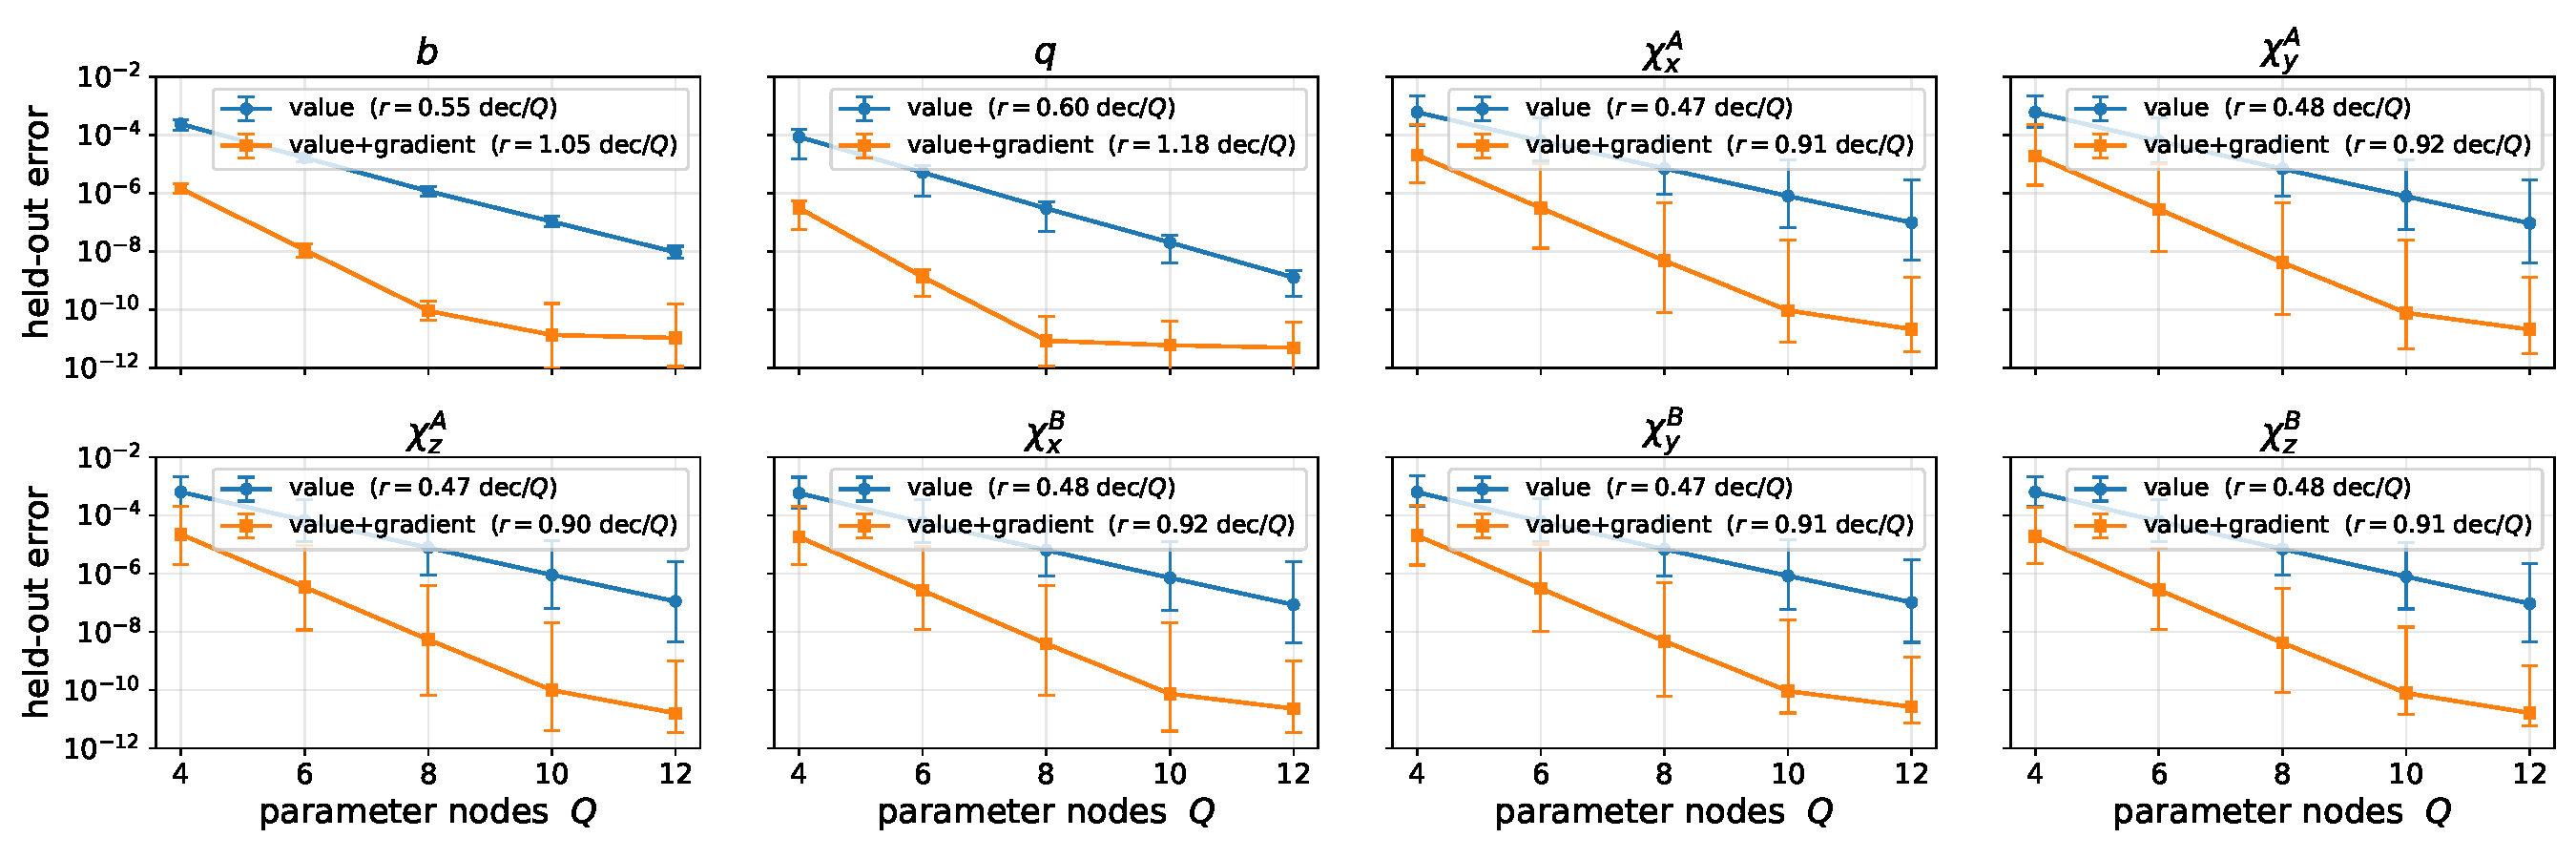
\includegraphics[width=\textwidth]{fig01_peraxis_hermite.pdf}
  \caption{\label{fig:peraxis}%
    \textbf{Per-axis convergence of the quasi-circular models.}
    Held-out interpolation error against the number of parameter nodes for each of
    the eight axes $(b,q,\boldsymbol{\chi}_A,\boldsymbol{\chi}_B)$; the first four
    are the four-dimensional aligned-spin model. The value-only surrogate is
    compared with the gradient-enhanced (Hermite) one, which also matches the
    certified parameter tangent at each node. Markers are medians over $100$
    random base points for the non-swept axes, with whiskers spanning the
    best--worst range. Every axis decays geometrically, at the rates fit from the
    median curves, and matching the tangent roughly doubles each rate
    (Sec.~\ref{sec:model:peraxis}).}
\end{figure*}

\subsection{Analyticity limits of the parameter map}
\label{sec:model:walls}

The convergence rate of a spectral parameter interpolant is set by the distance
from the sampling interval to the nearest singularity of the parameter-to-solution
map in the complex plane, through the \emph{Bernstein-ellipse} convergence bound
(Theorem~8.2 of Ref.~\cite{Trefethen2019}, going back to \cite{Bernstein1912}).
We map the sampling interval $[\theta_{\min},\theta_{\max}]$
of a parameter $\theta$ affinely onto $[-1,1]$ by
$\theta\mapsto\xi=(2\theta-\theta_{\max}-\theta_{\min})/(\theta_{\max}-\theta_{\min})$,
and consider the \emph{Bernstein ellipses} $E_\varrho$, which are defined as the ellipses in the complex
$\xi$-plane with foci at $\pm1$ whose semi-major and semi-minor axes sum to
$\varrho>1$. If the parameter-to-solution map is analytic inside $E_\varrho$, its $Q$-node Chebyshev interpolant
converges geometrically, with error $\sim\varrho^{-Q}$, i.e.\ a rate of $\log_{10}\varrho$
decades per node. The operative $\varrho$ is fixed by the \emph{largest} ellipse free
of singularities, so the nearest singularity of the map lies \emph{on} $E_\varrho$. A
singularity at the mapped point $\xi^\ast$ sits on the ellipse of parameter
$\varrho=|\xi^\ast+\sqrt{(\xi^\ast)^2-1}|$, which for a real singularity outside the
interval reduces to $\varrho=|\xi^\ast|+\sqrt{(\xi^\ast)^2-1}$. Hence, a singularity in parameter space close to the
sampled box $[\theta_{\min},\theta_{\max}]$ will yield a $\varrho$ just above unity and thus slow convergence, while a distant singularity will yield a
large $\varrho$ and fast convergence.

We read this estimate \emph{backwards} to locate the wall. From the slope of the
held-out error against the node count $Q$ we measure the geometric convergence rate
$r \equiv \log_{10}\varrho$, invert it to
$|\xi^\ast|=\tfrac12(\varrho+\varrho^{-1})$, and map $\xi^\ast$ back through the affine map, taking the real root outside the sampled box on the physically singular side
(small $b$ toward merger for the separation; large $|\chi|$ toward the extremal
limit for the spins), to read
off the inferred singularity location $\theta^\ast$. Sweeping the sampling range
then diagnoses the \emph{character} of the wall. A genuine real branch point stays
pinned at a fixed $\theta^\ast$ as the range changes. A complex-conjugate pair off
the real axis has no real singularity at all, yet the one-parameter fit still
returns a real $\theta^\ast$, the real point lying on the same Bernstein ellipse
as the true complex pair, which \emph{marches} outward as the range grows. The
legends of Fig.~\ref{fig:walls} report this inferred $\theta^\ast$ for each sampling
range alongside the fitted rate; whether $\theta^\ast$ holds still or recedes as the
range grows separates the two wall types below.

The quasi-circular family has two walls of opposite character
(Fig.~\ref{fig:walls}). Both sweeps are run at equal mass, with the remaining
parameters at their symmetric values.

The \emph{merger} wall, in the separation $b$, is hard. As the sampling interval
is pushed toward coincidence the rate degrades smoothly and tracks the Bernstein
prediction for a singularity fixed at $b=0$, the inferred $b^\ast$ staying at the
merger throughout. This resolves a concern specific to the orbiting family: the
$b\to0$ limit is \emph{doubly} singular --- the punctures coincide \emph{and} the
post-Newtonian tangential momentum $P_t\propto b^{-1/2}$ diverges --- yet the
extra branch does not \emph{relocate} the wall off $b=0$. Its only signature is a
mild undershoot of the measured rate below the pure-coincidence prediction at the
smallest $b_{\min}$: the momentum divergence makes the wall marginally
\emph{stronger}, not closer.

The \emph{spin} wall, in $\chi$, is by contrast soft. The measured rate degrades
only mildly as the range grows --- here deliberately extended past the production
box to locate the wall --- and the inferred nearest \emph{real} singularity
marches outward, staying beyond the sampled range throughout, which is the
signature of a complex-conjugate pair off the real axis rather than of a real
wall. That nearest feature is already super-extremal, well past the Cook--York
horizon-spin ceiling~\cite{CookYork1990}, so spin is a benign axis with no sharp
singularity near the physical box. What sets the convergence rate is therefore
the \emph{distance} of the nearest singularity and not its hardness: the family's
only hard wall lies on its fastest axis, while the slowest axes carry only soft,
receding ones.

\begin{figure*}[t]
  \centering
  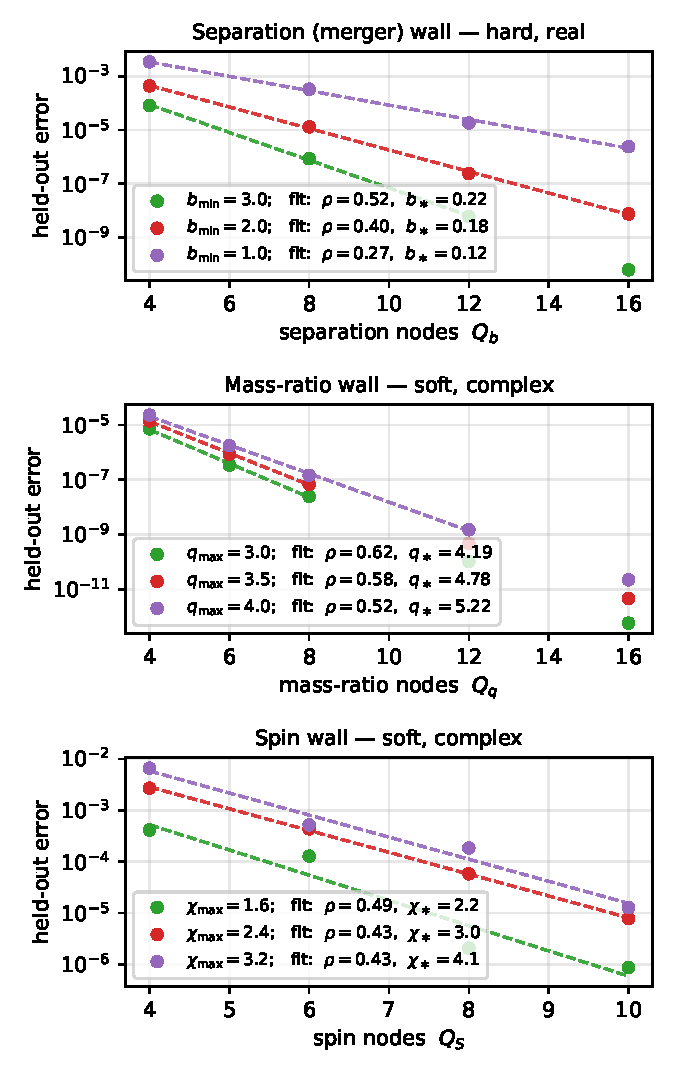
\includegraphics[width=\textwidth]{fig02_walls.pdf}
  \caption{\label{fig:walls}%
    \textbf{The two analyticity walls: separation (hard, real) versus spin (soft,
    complex).} Held-out interpolation error against the number of nodes along each
    axis, for a range of sampling intervals, with the geometric fit
    $\varepsilon\approx A\,10^{-\rho Q}$ overlaid (dashed). Each fit spans only
    the clean geometric window, so a dashed line stops short of the full node
    range wherever the error has already saturated on the float64 floor. Each
    legend entry gives, for its sampling range, the fitted rate $\rho$
    (decades/node) and the inferred nearest real singularity $\theta^\ast$.
    \emph{Left (merger wall, in the separation $b$):} the rate degrades as the
    interval is pushed toward coincidence while $\theta^\ast$ stays pinned at
    $b^\ast\approx0$ --- a hard real singularity fixed at the merger.
    \emph{Right (spin wall, in $\chi$):} the rate degrades only mildly and
    $\chi^\ast$ marches outward, remaining beyond the sampled range --- the
    signature of a complex-conjugate pair off the real axis
    (Sec.~\ref{sec:model:walls}).}
\end{figure*}

\subsection{Cost, memory, and certified residuals}
\label{sec:model:joint}

The offline cost of a full tensor grid scales as $\prod_k(Q_k{+}1)=O(Q^d)$; a
sparse (Smolyak) grid~\cite{Smolyak1963,NobileTemponeWebster2008} breaks this and is
what makes both the four-dimensional and the eight-dimensional quasi-circular
models (Sec.~\ref{sec:model:8d}) tractable. At isotropic Smolyak level $\ell=5$ the
four-dimensional model is $1105$ solver nodes and the eight-dimensional one
$15{,}713$ (field shape $45\times32\times8$), and the nested lower levels
$\ell=1\subset\cdots\subset5$ are fully contained in each corpus, so no level
costs additional solves. The offline saving is decisive: from the measured
per-axis rates, a tensor grid built to a \emph{bare} held-out accuracy of
$10^{-6}$--$10^{-9}$ would cost two to four orders of magnitude more solves ---
an accuracy the certified construction never needs, because the sparse grid
already supplies a Newton-basin warm start everywhere in the box and the polish
carries the correctness (the residual/field decoupling of
Sec.~\ref{sec:polish}). Even at matched per-axis resolution the comparison is
lopsided: a full tensor grid at the four-dimensional sparse grid's finest level
($33$ nodes per axis) would be $\sim\!10^3\times$ the sparse node count.

Evaluating the interpolant is cheap. A bare query is a single contraction over
the stored nodal solves, with no Newton iteration and no factorization, and costs
only a small fraction of one Newton--Krylov step of the elliptic solve --- less
still after the reduced-basis re-encoding of Sec.~\ref{sec:model:pod}. The warm
start it provides is therefore essentially free relative to the solve it seeds. A
certified query is that same warm-started solve, and its saving over a cold solve
is the reduced step count: two to four polish steps rather than the $\sim\!7$ a
cold start needs. The practical pattern is thus to bulk-generate initial data
with bare queries and certify only the configurations one actually evolves.
Because the model is nothing but its stored nodal solves, its memory is
\emph{linear} in the node count.

One distinction frames both models correctly: the \emph{bare} interpolant is a
warm start, not the product. Its joint held-out error falls geometrically with
the Smolyak level (Fig.~\ref{fig:joint}). The certified polish then makes even
that warm-start accuracy \emph{irrelevant to correctness}: a few Newton steps of the
genuine solver drive the constraint residual to $\|R\|_\infty\le10^{-10}$ at any
queried parameter (Fig.~\ref{fig:polish}), \emph{independent} of the
interpolation error, and they do so at \emph{every} one of the $1000$ random
off-node points tested, including the hard corners of the box where the bare
guess is poorest. The interpolant accelerates; the polish certifies.

\begin{figure*}[t]
  \centering
  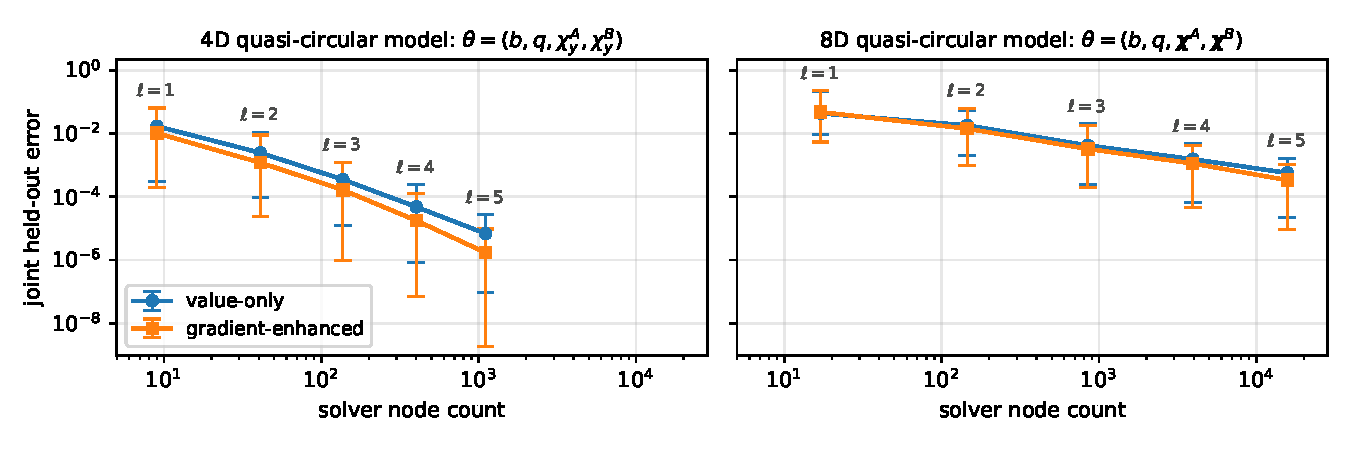
\includegraphics[width=\textwidth]{fig03_joint_dist.pdf}
  \caption{\label{fig:joint}%
    \textbf{Joint held-out convergence.} Joint held-out error over $1000$ random
    off-node points across Smolyak levels $\ell=1$--$5$, shown as the best,
    median, and worst of the distribution; every level is served from the
    committed corpus at the node counts shown, with no new solves.
    \emph{Left (four-dimensional model, $(b,q,\chi_{Ay},\chi_{By})$):} the bare
    sparse interpolant against the value$+$gradient$+$cross (full-bilinear
    Hermite--Smolyak) model enhanced on the two spin axes, which is more accurate
    at every level and reaches a $\sim\!35\times$ deeper best-case floor at the
    same node count, from the node tangents alone.
    \emph{Right (eight-dimensional general-spin model):} in preparation. The
    certified polish then drives every point to $\|R\|_\infty\le10^{-10}$
    (Fig.~\ref{fig:polish}).}
\end{figure*}

\begin{figure*}[t]
  \centering
  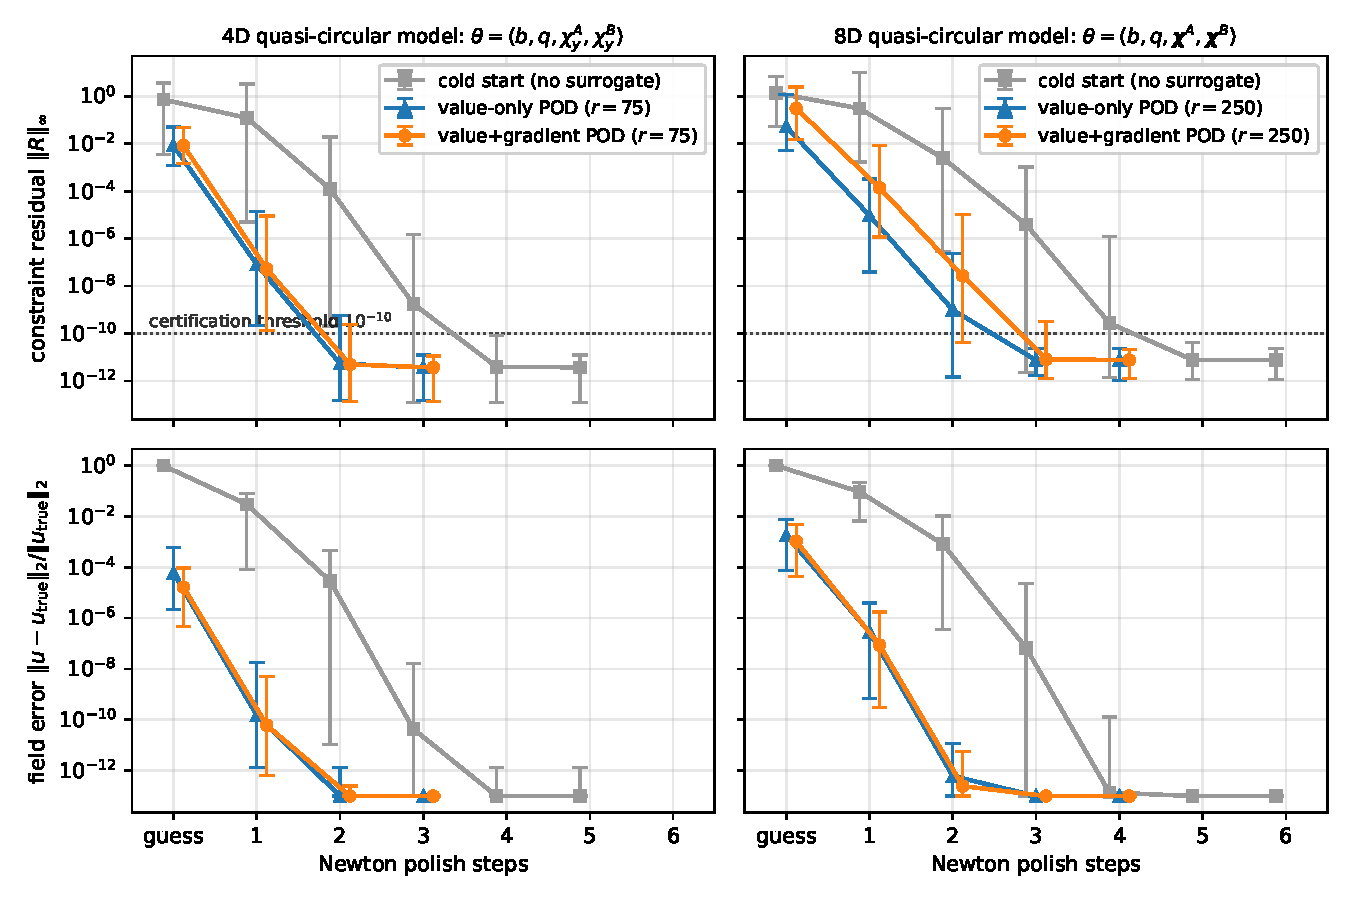
\includegraphics[width=\textwidth]{fig04_polish_staircase.pdf}
  \caption{\label{fig:polish}%
    \textbf{Certified refinement.} Constraint residual $\|R\|_\infty$ (top row)
    and relative field error $\|u-u_{\rm true}\|_2/\|u_{\rm true}\|_2$ (bottom
    row) over $1000$ uniformly-random off-node points of the quasi-circular models
    ($\chi$, $b\in[2,7]$, Smolyak $\ell=5$; left column four-dimensional
    aligned-spin, right column eight-dimensional general-spin), before the polish
    (``guess'') and after each Newton step. Each curve is the median with
    min--max whiskers over the $1000$ points, the field error measured against the
    converged certified iterate. \emph{Grey:} a surrogate-free \emph{cold start}
    from the solver's zero-field iterate, whose bare residual is
    $\mathcal{O}(1)$. \emph{Blue:} the value-only surrogate; \emph{orange:} the
    shipped gradient-enhanced (Hermite) surrogate, both POD-compressed to the same
    rank so that the two differ only in the gradient enhancement. Both surrogate
    warm starts certify \emph{every} point to $\|R\|_\infty\le10^{-10}$ in at most
    four steps, about two ahead of the cold start, \emph{independent} of the
    interpolation error. They are already field-accurate at the guess even though
    the residual there is orders of magnitude larger --- the decoupling of
    Sec.~\ref{sec:polish}.}
\end{figure*}

\paragraph*{Enlarging the enhanced set is counterproductive.}
Because the enhanced subspace is where the extra back-solves are spent, we tested
whether $\mathcal{E}$ should be enlarged beyond the two aligned-spin axes.
Extending it to all four axes of the aligned-spin box at the same level degrades
the held-out median by two orders of magnitude relative to doing nothing at all,
and completing the pairwise-bilinear crosses does not repair it. The degradation
is not an artifact of the reduced-basis compression, the cross layer, or the
one-dimensional Hermite operators, each of which we checked in isolation: swept
one axis at a time, Hermite beats Lagrange on \emph{every} axis. What correlates
is instead the \emph{number} of simultaneously enhanced axes --- enhancing any
single axis improves on value-only, two degrade, and four degrade badly ---
consistent with cancellation in the Smolyak combination being governed by the
one-dimensional operator norms, which multiply over the enhanced dimensions while
the accuracy gain enters only once per axis. We have not established that
mechanism directly. The practical consequence is that $\mathcal{E}$ should be
kept small and spent on the slowest axes, and that the shipped
$\mathcal{E}=\{\chi_{Ay},\chi_{By}\}$, completed to full bilinear, is at or near
the optimum of the configurations we measured.

\subsection{The eight-dimensional general-spin model}
\label{sec:model:8d}

Promoting the two aligned spins to full vectors takes the model to eight
dimensions, $\theta=(b,q,\boldsymbol{\chi}_A,\boldsymbol{\chi}_B)$, where the
tensor grid's $Q^d$ cost makes the Smolyak construction of
Sec.~\ref{sec:param:smolyak} not merely advantageous but necessary. The method is
unchanged: with the in-plane spin axes centred on zero, the four-dimensional
aligned model nests, node-for-node, inside the eight-dimensional one, and the
$\ell=5$ grid is $15{,}713$ solver nodes --- reusing the entire aligned corpus and
adding only the genuinely-new precessing nodes. Its in-plane spin axes converge
like the aligned ones and show the same cross-hole equalization that
$\chi$-sampling buys (Fig.~\ref{fig:peraxis}), and the in-plane spin wall is again
soft, its nearest real singularity receding as the fit range grows, so precession
introduces no new hard wall. At this dimension it is the polish, not the bare
sparse interpolant, that carries the accuracy: the $1000$-point certified-polish
statistics for both $\ell=5$ models are reported in Fig.~\ref{fig:polish}. The
gradient-enhanced corpus reduced-basis compresses by a factor of $27$ with no loss
of certification or differentiability (Sec.~\ref{sec:model:pod}).

\subsection{Reduced-basis compression of the model}
\label{sec:model:pod}

The corpora are correspondingly large: the gradient-enhanced four-dimensional
$\ell=5$ corpus (values \emph{and} node tangents) is $486$~MiB and the
eight-dimensional one $12.1$~GiB. This is a distribution liability for an artifact
meant to be hosted and cited, and it is entirely removable by the reduced-basis
(POD) re-encoding of Sec.~\ref{sec:param:pod}: an SVD of the stored fields yields
orthonormal spatial modes $\Phi$, of which we keep the leading $r$ and interpolate
the length-$r$ coefficient vector at each node in place of the full field. The
singular values decay geometrically (the map is analytic in $\theta$, as in
Sec.~\ref{sec:model:walls}): for the four-dimensional model the rank-$r$
reconstruction error of the corpus falls below $10^{-6}$ by $r=87$ modes, and
because the value and its parameter tangents \emph{share} one spatial basis, the
enhanced corpus needs only some $12\%$ more modes than the value-only one at the
same tail. The rank at a fixed accuracy is set by the intrinsic dimension of the
solution manifold, not by the sampling density: it is the counterpart to
Sec.~\ref{sec:param:smolyak} along the orthogonal axis --- the Smolyak level fixes
the parameter resolution and the offline solve count, POD the spatial rank, and
the two are independent.

Figure~\ref{fig:pod} shows the resulting memory--accuracy tradeoff. At the shipped
ranks the four-dimensional model shrinks by a factor of $42$ ($486$~MiB to
$11.5$~MiB) and the eight-dimensional one by $27$ ($12.1$~GiB to $461$~MiB), and
per-query evaluation, now a barycentric sum over $r$ coefficients rather than the
full field, drops to a few milliseconds. The certified constraint residual, the
number of Newton steps needed to reach it (Sec.~\ref{sec:polish}), and the
verified $\dID$ (Sec.~\ref{sec:param:diff}) are all preserved: the mode projection
loses only the truncation-tail fraction of the gradient, and the compressed model
reproduces the truncated interpolant to that tail and reloads as a standalone
predictor. The decomposition is computed once from the existing corpus, in minutes
and with no new solves.

Three further compressions stack on top, all computed from the same corpus with no
new solves, and all preserving the certified Newton-step count and the parameter
gradient: single-precision storage of the spatial modes, an anisotropic Smolyak
grid weighted toward the slowly-converging spin axes, and a per-Fourier-mode basis
that stores the dominant $m=0$ block in its compact form rather than the
$8\times$-redundant nodal one. Together they reduce even the eight-dimensional
model several-fold further.

\begin{figure*}[t]
  \centering
  
\includegraphics[width=\textwidth]{fig05_guess_vs_memory.pdf}
  \caption{\label{fig:pod}%
    \textbf{Reduced-basis (POD) compression versus stored memory.} Constraint
    residual $\|R\|_\infty$ of the bare barycentric guess (top row) and the
    relative field error $\|u-u_{\rm true}\|_2/\|u_{\rm true}\|_2$ of the
    \emph{same} guess against the certified solve (bottom row), as the POD
    truncation rank $r$ is swept. Median line with min--max whiskers over
    uniformly-random off-node query points; each point is labelled by $r$ and
    $\star$ marks the full-rank model. Columns share the memory axis:
    \emph{left,} the four-dimensional quasi-circular model; \emph{right,} the
    eight-dimensional general-spin model (Sec.~\ref{sec:model:8d}), whose
    field-error sweep is pending. Compressing raises the bare-guess residual, but
    this warm-start quality is irrelevant to correctness: the certified polish
    (Sec.~\ref{sec:polish}) drives every query to $\|R\|_\infty\le10^{-10}$ in the
    same Newton-step count regardless. The field error meanwhile \emph{saturates}
    at a far lower rank than the residual, so the redundancy discarded by
    compression is exactly the high-derivative content the residual amplifies and
    the field norm cannot see (the decoupling of Sec.~\ref{sec:polish}). At the
    shipped ranks the models shrink $42\times$ and $27\times$ at no cost to the
    certified output.}
\end{figure*}

\subsection{External validation}
\label{sec:model:validation}
The underlying initial data reproduce the established
TwoPunctures~\cite{AnsorgBruegmannTichy2004} solver to spectral accuracy on the
most demanding, genuinely non-axisymmetric configurations, and they are
evolution-ready: on an evolution grid their finite-difference constraint violation
is indistinguishable from TwoPunctures-sourced data. Because certification is an
\emph{internal} guarantee (Sec.~\ref{sec:polish}), this agreement is credibility
rather than the correctness claim itself; Appendix~\ref{sec:validation} gives the
full comparison.

% ===========================================================================
\section{Applications}
\label{sec:applications}
% ===========================================================================
The two payoffs of the method are that it is differentiable and
constraint-certified, and we
demonstrate both in two applications: certified parameter targeting on the
flagship four-dimensional quasi-circular model, and eccentricity reduction on a
purpose-built two-dimensional $(b,P_t)$ model. Each targets
a standard numerical-relativity initial-data workflow, and in each the honest cost
metric is the number of \emph{certified} elliptic solves.

\subsection{Certified parameter targeting}
\label{sec:applications:targeting}

The first workflow is parameter control~\cite{Mendes2025}: find the free data that
realize a chosen physical configuration. The standard tool is a black-box control
loop, i.e.\ an outer Newton/Broyden iteration that adjusts the free data and performs a
full constraint solve at every step to measure the resulting physical parameters. We
target the ADM mass and angular momentum $(\Madm,J)$ by adjusting $(b,q)$, over $100$
random known-answer targets, and compare three strategies. A \emph{cold} black box
solves the constraints from scratch at each control evaluation. A \emph{warm} black
box seeds each solve from the interpolant, so every constraint solve begins close to
its answer. The \emph{differentiable} method runs the entire Gauss--Newton control
loop on the free surrogate using the analytic $\partial F/\partial\theta$, then certifies the
result with a few Newton steps (i.e.\ no
elliptic solve per step, and no finite-difference Jacobian).

Differentiability changes the cost class here
(Fig.~\ref{fig:targeting}). The gradient method reaches every target in a
\emph{fixed} three certified solves, independent of target difficulty, whereas both
black-box variants take a target-dependent median of ten.
Warm-starting cuts the per-solve cost but \emph{not}
the number of solves: the outer control iteration is unchanged, so a warm start alone
never leaves the black box's complexity class. The distinction is structural. A
black-box loop can drive the residual to zero only through function evaluations, and
each one is a certified elliptic solve; a low-rank Jacobian update (Broyden's method,
which sidesteps the $d$ extra solves a finite-difference Jacobian would cost) lowers
the iteration count but cannot remove the one solve per iteration. The analytic
gradient removes those per-iteration solves outright, running the search entirely on
the free surrogate and leaving only the last-mile certification, a saving that
widens with the number of controlled parameters.

\begin{figure}[t]
  \centering
  
\includegraphics[width=\columnwidth]{fig06_targeting.pdf}
  \caption{\label{fig:targeting}%
    \textbf{Certified parameter targeting.} Reaching a physical target
    $(\Madm,J)$ by adjusting $(b,q)$, over $100$ random known-answer targets,
    measured in \emph{certified} elliptic solves. Each method is drawn as the
    across-target median residual at each solve count, with min--max whiskers.
    Running the control loop on the free surrogate with the parameter gradient
    reaches tolerance in at most three certified solves for every target; the
    black-box loop takes a target-dependent median of ten.}
\end{figure}

\subsection{Eccentricity reduction}
\label{sec:applications:ecc}

The second workflow is eccentricity control, the most common tuning step in
preparing quasi-circular data. We use the Cook effective-potential
method~\cite{Cook1994}: along a sequence of fixed angular momentum $J$ (radial
momentum $P_r=0$, i.e.\ an apsis), the binding energy $E_b=\Madm-(M_A+M_B)$ has a minimum at the circular orbit
$\partial E_b/\partial b|_J=0$, and a mildly off-circular apsis at $(b_0,J)$ has
eccentricity $e=|b_0-b'|/(b_0+b')$ set by the second turning point $b'$ across that
minimum. Reducing eccentricity is driving $b_0\to b_{\rm circ}$.

The classical method locates $b_{\rm circ}$ by \emph{scanning} $b$ at fixed $J$, i.e.\
one certified solve per point, and fitting the minimum. This workflow needs the
tangential momentum $P_t$ as a \emph{free} axis (one scans $b$ at fixed
$J=2bP_t$), which the quasi-circular model of Sec.~\ref{sec:model} deliberately
does not carry; we therefore build a dedicated small two-dimensional surrogate in
$(b,P_t)$ (equal mass, no spin) by the identical machinery of
Secs.~\ref{sec:param}--\ref{sec:model}. On it the differentiable binding energy
exposes $\partial E_b/\partial b|_J$ analytically, so a Newton root-find locates the
circular orbit on the free interpolant and certifies at the end. Sweeping $J$
traces the circular-orbit sequence, whose minimum shifts outward with angular
momentum (Fig.~\ref{fig:ecc}). The gradient locates each $b_{\rm circ}$ in three
certified solves against the scan's thirteen, agreeing with it to
$5\times10^{-3}$ where the well is well resolved. It is moreover \emph{more
accurate} in the shallow, near-innermost-stable-orbit regime, where the fixed
thirteen-point scan mislocates the minimum by half a mass and the derivative still
resolves it: a black-box scan must sample ever more finely, at more certified
solves, exactly where the physics is most delicate. The same differentiable $E_b$
reads the orbital eccentricity off the turning points, from $e=0$ at the circular
orbit to $e\approx0.23$ at the box edge, and so exposes
$\partial e/\partial\theta$ for gradient-based eccentricity reduction.

\begin{figure}[t]
  \centering
  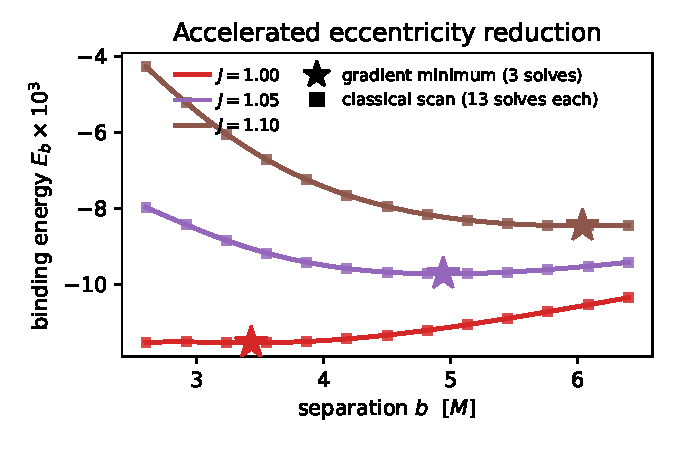
\includegraphics[width=\columnwidth]{fig07_eccentricity.pdf}
  \caption{\label{fig:ecc}%
    \textbf{Accelerated eccentricity reduction.} At fixed angular momentum $J$ the
    binding energy $E_b(b)$ has a minimum at the circular orbit; sweeping $J$ the
    minimum shifts outward, tracing the circular-orbit sequence. For each $J$ the
    differentiable $\partial E_b/\partial b$ locates that minimum in three certified
    solves (stars), against the classical certified-solve scan's thirteen (squares).
    In the shallow small-$J$ well the fixed scan mislocates the minimum, whereas the
    derivative still resolves it.}
\end{figure}

Both workflows make the same point: the differentiable, certified map turns a
black-box search (a control loop and an effective-potential scan) into a gradient
problem solved on the free surrogate and certified in a handful of Newton steps,
where the black box instead pays a full certified elliptic solve at every trial.

% ===========================================================================
\section{Discussion and conclusions}
\label{sec:conclusions}
% ===========================================================================
We have introduced a parametric solver for binary-black-hole puncture initial data
that combines sparse interpolation with Newton refinement. The interpolation
supplies an inexpensive parameter-dependent initial guess, while the subsequent
elliptic solve certifies every returned datum to a prescribed constraint tolerance.
Because the construction is implemented in JAX, the resulting parameter-to-solution
map is also exactly differentiable with respect to the physical parameters. The
four-dimensional aligned-spin and eight-dimensional general-spin models demonstrate
that this construction remains practical across physically relevant
binary-black-hole parameter spaces, while the parameter-targeting and
eccentricity-reduction examples show how its derivatives can reduce the number of
certified elliptic solves required in downstream workflows.

The two headline models are genuinely three-dimensional, quasi-circular parametric
surrogates spanning the aligned- and general-spin families (Sec.~\ref{sec:model}).
What remains is scope, not a barrier of principle. The most natural extension is
\emph{eccentricity}: relaxing the quasi-circularity condition to carry an
independent radial momentum adds one axis on top of the orbiting family, by the same
machinery --- indeed we already build a small $(b,P_t)$ eccentricity model this way
(Sec.~\ref{sec:applications:ecc}). The parametric, certified, and differentiable
machinery is \emph{dimension-agnostic}, i.e.\ it sees only a
$\texttt{solve}(\theta,\text{guess})$ routine and an optional tangent, so each
extension is a change of solver and box, not of method.

One limitation is inherited from the free data themselves, not from the
parametric method. Bowen--York, conformally flat data carry spurious (``junk'')
radiation that the early evolution must shed~\cite{Lovelace2009}, and cannot
represent near-extremal black holes: the \emph{horizon} spin of a Bowen--York
puncture saturates at $\chi\approx0.93$ no matter how large the free-data spin
parameter~\cite{CookYork1990,DainLoustoZlochower2008}, which is why
nearly-extremal-spin simulations use conformally curved (e.g.\ superposed
Kerr--Schild) initial data~\cite{Lovelace2008}. Within the moving-puncture
mainstream ($\chi\lesssim0.9$) the family built here is the standard input; and
because the parametric layer is solver-agnostic
(Sec.~\ref{sec:param:build}), a conformally-curved solver could be swapped in
under the same interpolation, certification, and compression machinery.

Two accuracy caveats are worth stating explicitly. First, the spin-wall analysis
is quantitative only within the physical range ($\chi_{\max}\lesssim0.8$): pushing
the sampling interval toward and past extremal spin mixes the genuine (complex,
far) singularity with pre-asymptotic and spatial-floor effects, so the clean
single-$\chi^\ast$ characterization is reported for the physical regime, not
extrapolated beyond it. Second, the certified $\|R\|_\infty\le10^{-10}$ gate is
verified at the production grid ($44\times32\times8$); at higher meridian
resolution the whole-field equilibrated residual floors higher, because the stiff
$m^2/\rho^2$ term amplifies roundoff in the azimuthal modes that carry no source
content, while the physically populated modes stay three orders of magnitude
below. The floor is therefore set by empty modes rather than by the physics, and
the certification tolerance should be read at the grid it is quoted for.

Finally, beyond the immediate use cases, the method produces exactly the kind of
object a broader surrogate or foundation-model programme for binary-black-hole
spacetimes needs at its base: a fast, \emph{exact} (constraint-certified), and
\emph{differentiable} initial-data generator across a physical parameter space.
Such a generator can serve as a certified training source and a warm-start oracle
for those models, supplying gradients $\dID$ for end-to-end parameter inference.

% ===========================================================================
\begin{acknowledgments}
The authors would like to thank Miguel Bezares Figueroa, Thiago Assump\c{c}\~ao, and Ignacio Brevis for encouraging and interesting discussions.
This research was supported by the Research Foundation -- Flanders (FWO; Grant No.\ I000725N and I002123N).
\end{acknowledgments}

\appendix


% ===========================================================================
\section{Validation against TwoPunctures}
\label{sec:validation}
% ===========================================================================
A surrogate is only as trustworthy as the data it reproduces, so we validate the
underlying initial data against the established TwoPunctures code~\cite{AnsorgBruegmannTichy2004}, specifically its standalone C port from the NRPy
suite, compiled against GSL.
The comparison is genuine: TwoPunctures discretizes with a
Chebyshev$^2\times$Fourier grid, PARASOL with the prolate single patch of
Sec.~\ref{sec:solve:abt}, so agreement is a statement about the physical solution,
not a shared discretization. We lead with the most demanding, genuinely
non-axisymmetric configurations the quasi-circular model relies on
(Appendix~\ref{sec:validation:3d}), then the quasi-circular data itself
(Appendix~\ref{sec:validation:qc}) and its evolution-readiness
(Appendix~\ref{sec:validation:constraints}); the axisymmetric limit, where both codes
reduce to their $m=0$ core and the agreement deepens to machine precision.


\subsection{Non-axisymmetric validation}
\label{sec:validation:3d}

The quasi-circular model of Sec.~\ref{sec:model} is genuinely non-axisymmetric, so
its credibility rests on validating the three-dimensional (Fourier-in-$\phi$)
solver of Sec.~\ref{sec:solve:abt} against TwoPunctures. We do so on
non-axisymmetric configurations that isolate the ingredients the orbiting data
combine --- an off-axis (transverse) momentum component and a misaligned spin ---
and on the genuinely three-dimensional observable, the ADM angular momentum, on
which the quasi-circular family relies.

For a misaligned-spin slice ($|S_A|=0.3$ tilted $56.3^\circ$ off the collision
axis, i.e.\ along $(0.3,0,0.2)$; axial momentum $P=0.5$, $b=1.5$), the conformal
factor converges spectrally to TwoPunctures, $\max|\psi-\psi_{\rm TP}|$ falling by
an order of magnitude over the resolution ladder to $1.7\times10^{-7}$ and still
decreasing at the top of the ladder (Fig.~\ref{fig:3dval}); this $\sim\!10^{-7}$
floor is resolution- rather than solver-limited (one order above the two-centre
axisymmetric floor), and the certified polish of Sec.~\ref{sec:polish} recovers
$\|R\|_\infty\le10^{-10}$ regardless. The azimuthal content decays exponentially in
$m$ (Fig.~\ref{fig:3dval}b): a misaligned spin populates
$|\hat u_1|/|\hat u_0|\sim2$--$5\%$ with $\sim\!2$ decades of decay by $m=3$, while
\emph{aligned} spin leaves every $m\!\ge\!1$ mode at machine zero --- a hard
numerical confirmation that aligned spin is axisymmetric and that a handful of
Fourier modes resolve a minimal break. Across a $b\times|S|\times\theta_S$ grid of
$45$ slices the certified Newton--Krylov residual floor is uniform and small
(median $6.6\times10^{-12}$, worst $1.8\times10^{-11}$), never degrading
systematically with spin tilt or separation.

While the pointwise field floors at $\sim\!10^{-7}$ in this hardest
(misaligned-spin) case, the \emph{integral} quantities agree to machine precision
even in three dimensions. The total ADM mass matches TwoPunctures to
$\sim\!10^{-12}$ on off-axis-momentum data (where the mode iteration is the full
Newton). The genuinely three-dimensional observable, the ADM angular momentum,
is computed from the conformal Bowen--York tensor by a York surface integral and
cross-checked against the closed form $J^i=\sum_X(S_X^i+(x_X\times P_X)^i)$ and
against TwoPunctures (Fig.~\ref{fig:tpval}): for pure spin the ADM-$J$ tilt off the
collision axis equals the spin tilt to machine precision across all magnitudes and
separations; an anti-symmetric off-axis momentum $P_x$ produces an orbital
$J_y=2b\,P_x$ recovered exactly by the surface integral; and agreement with the
TwoPunctures-reported $J$ (rotated to the common frame) is at the level of the
analytic Gauss law on both sides, $\le1.4\times10^{-14}$. In the axisymmetric limit
the field agreement itself deepens to machine precision --- two independently
discretized spectral codes agreeing on $\psi$ to $4.7\times10^{-12}$ and on the
total ADM mass to a relative $1.0\times10^{-11}$ (equal-mass slice $b=3$, axial
$P=0.5$) --- which we quote as the deepest code-to-code anchor rather than as a
separate axisymmetric study.

\begin{figure*}[t]
  \centering
  
\includegraphics[width=\textwidth]{fig08_3d_validation.pdf}
  \caption{\label{fig:3dval}%
    \textbf{Non-axisymmetric data validated against TwoPunctures.}
    \emph{Left:} for a misaligned-spin slice ($S_A=(0.3,0,0.2)$, $b=1.5$,
    $P=0.5$), the conformal factor converges spectrally to TwoPunctures
    ($\max|\psi-\psi_{\rm TP}|$, dashed), still decreasing at the top of the
    resolution ladder, while the certified Newton--Krylov residual $\|R\|_\infty$
    (solid) is near machine precision at the production resolution. Its slow rise
    at higher meridian resolution is the empty-high-$m$-mode roundoff
    amplification of Sec.~\ref{sec:conclusions}, a norm artifact rather than a
    solver limitation: the field keeps converging throughout.
    \emph{Right:} the azimuthal $\phi$-mode spectrum of the solved field decays
    exponentially in $m$, and aligned spin ($\theta_S=0$) leaves every
    $m\!\ge\!1$ mode at machine zero, confirming that few Fourier modes resolve a
    minimal break of axisymmetry.}
\end{figure*}

\begin{figure*}[t]
  \centering
  
\includegraphics[width=\textwidth]{fig09_tp_validation.pdf}
  \caption{\label{fig:tpval}%
    \textbf{TwoPunctures validation: the three-dimensional observable and the
    quasi-circular data.}
    \emph{(a)} For pure spin the ADM-$J$ tilt off the collision axis tracks the
    spin tilt exactly ($J=\sum_X S_X$): all magnitudes collapse onto
    $\theta_J=\theta_S$, with the TwoPunctures anchors (stars) on the line.
    \emph{(b,c)} On a quasi-circular slice ($b=4$, $q=1$, no spin) the conformal
    factor converges spectrally to TwoPunctures, saturating at the two-centre
    spatial floor, while the ADM mass converges some three orders of magnitude deeper
    still --- the boundary-spectral $\Madm$ outrunning the pointwise field.}
\end{figure*}

\subsection{Quasi-circular data against TwoPunctures}
\label{sec:validation:qc}

The headline check is that the quasi-circular initial data itself reproduces the
oracle. The frame convention (risk R2) is fixed first: the separation is along $z$
and the quasi-circular tangential momentum along $x$, so the orbital angular
momentum is along $+y$; the proper rotation taking the PARASOL frame to
TwoPunctures maps PARASOL-$y$ to TP-$z$, and ``aligned spin'' therefore means the
$S_y$ component. With the convention fixed, the momentum condition is honest: the
closed-form tangential momentum approaches the Newtonian value,
$P_t/[\mu\sqrt{M/2b}]\to1$ as $b$ grows (from $1.59$ at $b=2$ to $1.016$ at
$b=64$), and the radial component vanishes, $P_r/P_t\to0$ (as $b^{-5/2}$), so
``quasi-circular'' is quantitatively justified. The field and mass converge to the
oracle (Fig.~\ref{fig:tpval}b,c): on a quasi-circular slice ($b=4$, $q=1$, no spin) the conformal factor
converges spectrally to TwoPunctures, $\max|\psi-\psi_{\rm TP}|$ reaching
$1.7\times10^{-9}$ at $64\times44$ (the two-centre spatial floor), and the total
ADM mass agrees with the TwoPunctures energy to $5.8\times10^{-12}$ --- the
boundary-spectral $M_{\rm ADM}$ converging far deeper than the pointwise field.
Finally, the closed-form angular momentum $J=2b\,P_t+S_{Ay}+S_{By}$ (along $+y$)
equals the frame-rotated TwoPunctures ADM $J$ to machine precision, with net linear
momentum $P_A+P_B=0$ exactly; since the Bowen--York $J$ is analytic in the free
data on both sides, this pins the frame convention and momentum wiring (retiring
risk R2) rather than measuring the field.

\subsection{Evolution-readiness on an evolution grid}
\label{sec:validation:constraints}

The oracle-independent test of evolution-readiness is to interpolate the spectral
initial data onto a uniform Cartesian grid --- as an evolution code would ingest it
--- and measure the residual constraint violation with a \emph{generic}
finite-difference Hamiltonian and momentum constraint monitor (FD Christoffels and
Ricci, no conformal-flatness shortcut), exactly as a free-evolution code's
diagnostics would~\cite{BaumgarteShapiro2010}. On the equal-mass head-on base
case both constraints converge at the expected second order in the grid spacing
$h$ (measured orders $2.14$ for $\|H\|_2$ and $2.02$ for $\|M\|_2$). Critically,
feeding the \emph{TwoPunctures}-sourced $\psi$ through
the identical monitor on the same grid gives a violation identical to all recorded
digits (the two $\psi$ fields differ far below the truncation-dominated norms) ---
so the residual is genuine finite-difference truncation, not a defect of the
PARASOL data, and PARASOL initial data is as evolution-ready as TwoPunctures'.
Equivalently, the spatial resolution used here is \emph{not} the accuracy-limiting
factor for a numerical-relativity evolution: the initial-data spectral error lies
well below the finite-difference truncation of any practical evolution grid, so the
elliptic solve is already resolved beyond what the downstream evolution can
register, and the certified polish guarantees $\|R\|_\infty\le10^{-10}$ on the
emitted datum in any case.


% ===========================================================================
\section{Verification of the parameter sensitivities}
\label{sec:app:tangent}
% ===========================================================================
The verification proceeds in two stages, because two distinct statements are at issue:
that Eq.~\eqref{eq:tangent} is the sensitivity of the certified solve, and that the
gradient the surrogate exposes is that same sensitivity.

Table~\ref{tab:tangent3d} settles the first on the production three-dimensional
operator, comparing the tangent of Eq.~\eqref{eq:tangent} against central finite
differences of the certified Newton--Krylov solve itself. The two agree to
$\sim\!10^{-9}$ on every axis of the aligned-spin box, at the accuracy of the
finite-difference oracle, so the analytic $\partial R/\partial\theta_k$ and the
back-solve reproduce the true derivative of the certified map.

Table~\ref{tab:tangent} settles the second. Automatic differentiation of the surrogate
agrees with central finite differences of that same surrogate to
$10^{-10}$--$10^{-9}$, which verifies the differentiation itself but says nothing about
certification. The load-bearing column is the last one: the exposed gradient reproduces
the independently computed tangent of Eq.~\eqref{eq:tangent} to $\sim\!2\times10^{-7}$
along the spin axes and $\sim\!10^{-5}$ along $b$ and $q$. That residual is the
interpolation error of the derivative, not an error in either object, and it is largest
along $b$ and $q$ for the same reason the field interpolation is slowest there
(Sec.~\ref{sec:model:peraxis}); it decreases exponentially with the parameter order.

\begin{table}[t]
  \caption{\label{tab:tangent3d}%
    \textbf{The tangent of Eq.~\eqref{eq:tangent} against the certified solve.} Maximum
    relative difference between the implicit-function-theorem tangent
    $\partial U/\partial\theta_k$, obtained from one back-solve against the factored
    Jacobian, and second-order central finite differences of the certified
    Newton--Krylov solve with step $h$. Non-axisymmetric quasi-circular slice at
    $b=2.4$, $q=1.7$, $P_t=0.5$, $\chi_{Ay}=0.30$, $\chi_{By}=0.20$, on the
    $(N_A,N_B,N_\phi)=(18,14,6)$ grid; both solves are certified to
    $\|R\|_\infty=2.4\times10^{-14}$.}
  % generated by tab01_tangent_operator_tex.py from tabdata/tab01_tangent_operator.json — do not edit by hand
\begin{ruledtabular}
\begin{tabular}{lcc}
  Axis $\theta_k$ & $h$ & Eq.~\eqref{eq:tangent} vs.\ finite differences \\
  \colrule
  $b$ & $10^{-4}$ & $1.9\times10^{-9}$ \\
  $q$ & $10^{-4}$ & $2.7\times10^{-9}$ \\
  $\chi^{A}_{y}$ & $10^{-4}$ & $7.3\times10^{-9}$ \\
  $\chi^{B}_{y}$ & $10^{-4}$ & $5.6\times10^{-9}$ \\
\end{tabular}
\end{ruledtabular}

\end{table}

\begin{table}[t]
  \caption{\label{tab:tangent}%
    \textbf{The exposed sensitivity against both references.} Maximum relative
    difference between the automatic-differentiation sensitivity
    $\partial U/\partial\theta_k$ of the surrogate and, respectively, second-order
    central finite differences of the same surrogate with step $h$, and the
    implicit-function-theorem tangent of Eq.~\eqref{eq:tangent} computed independently
    from the certified solve at the same parameter point. Two-centre aligned-spin
    interpolants on the $(N_A,N_B)=(36,24)$ grid at $M=1$: a $(b,q)$ model of order
    $Q=(12,10)$ over $b\in[3,12]$, $q\in[1,3]$, evaluated off-node at
    $(b,q)=(6.337,1.713)$; and a $(\chi_A,\chi_B)$ model of order $Q=8$ over
    $[0,0.6]^2$ at fixed $q=1.5$, $b=4$, evaluated off-node at
    $(\chi_A,\chi_B)=(0.413,0.227)$, where $\chi_A$ and $\chi_B$ are the aligned-spin
    magnitudes on the two punctures. The reference solves are certified to
    $\|R\|_\infty\le2\times10^{-12}$.}
  % generated by tab02_tangent_surrogate_tex.py from tabdata/tab02_tangent_surrogate.json — do not edit by hand
\begin{ruledtabular}
\begin{tabular}{lccc}
  Axis $\theta_k$ & $h$ & vs.\ finite differences & vs.\ Eq.~\eqref{eq:tangent} \\
  \colrule
  $b$ & $10^{-6}$ & $5.5\times10^{-9}$ & $1.3\times10^{-5}$ \\
  $q$ & $10^{-6}$ & $4.4\times10^{-10}$ & $1.2\times10^{-5}$ \\
  $\chi^{A}_{y}$ & $10^{-6}$ & $2.0\times10^{-10}$ & $1.7\times10^{-7}$ \\
  $\chi^{B}_{y}$ & $10^{-6}$ & $2.0\times10^{-10}$ & $1.8\times10^{-7}$ \\
\end{tabular}
\end{ruledtabular}

\end{table}

\bibliographystyle{apsrev4-2}
\bibliography{references}

\end{document}
